% Main LaTeX document for the RSS'09 Booklet
\documentclass[9pt, twoside, openany]{extbook}


\usepackage{ifthen}

%define to switch between different flavours:
\def \targetoutput {print}  %generate for printing (no colored hyperlinks, pages are all upright)
%\def \targetoutput {usbstick} %optimized for screen viewing, pre-rotated landscape pages, links to local files
%\def \targetoutput {online}

\usepackage{fleqn}
%\usepackage{latexpackages/my}
\usepackage{times}
\usepackage[normalem]{ulem}
\usepackage{eurosym}
\usepackage{setspace}
\usepackage{graphicx}
\usepackage{epstopdf}
%\usepackage{epsfig}
%\newcommand{\denselist}{\itemsep -3pt\topsep 0pt\partopsep 0pt\parsep 0pt}

\usepackage[a4paper,top=3cm, left=1.5cm, right=1.5cm, bottom=2.5cm, headsep=1.5cm, footskip=8mm]{geometry}
\setlength{\headheight}{34pt} %adjust headheight to suppress warnings

%\pdfoutput=0
\usepackage{wrapfig,graphicx}
\usepackage{hyperref}


\ifthenelse{\equal{\targetoutput}{print}}{
  \hypersetup{bookmarksopen,bookmarksnumbered,
  pdfpagemode=UseOutlines,
  colorlinks=true,
  linkcolor=black,
  anchorcolor=black,
  citecolor=black,
  filecolor=black,
  menucolor=black,
  urlcolor=black,
  debug=true
  }
}{
  \hypersetup{bookmarksopen,bookmarksnumbered,
  pdfpagemode=UseOutlines,
  colorlinks=true,
  linkcolor=blue,
  anchorcolor=blue,
  citecolor=blue,
  filecolor=blue,
  menucolor=blue,
  urlcolor=blue,
  }
}

\usepackage[utf8]{inputenc}
\usepackage[english]{babel}
\usepackage{array}
\usepackage{wrapfig}

\DeclareGraphicsExtensions{.pdf,.jpg, .png}

\usepackage[usenames,dvipsnames]{xcolor}
%\definecolor{RSSorange}{HTML}{F2531B}
\definecolor{RSSblue}{HTML}{002654}

%\usepackage[table]{xcolor}
\usepackage{tabularx}
\newboolean{include-notes}
\setboolean{include-notes}{true}

% http://en.wikibooks.org/wiki/LaTeX/Colors
\newcommand{\adnote}[1]{\ifthenelse{\boolean{include-notes}}%
 {\textcolor{LimeGreen}{\textbf{NOTE: #1}}}{}}

 
\ifthenelse{\equal{\targetoutput}{print}}{\usepackage{lscape}}{\usepackage{pdflscape}} %don't load pdflscape for print version

\ifthenelse{\equal{\targetoutput}{usbstick}}{
    \newcommand{\linkedfile}[2]{\href{#2}{#1}} %\linkedfile{this file}{path/filename}
}{
    \newcommand{\linkedfile}[2]{#1}
}


%these are for the fancy general schedule:
\usepackage{latexpackages/timetable}
\usepackage{colortbl}

 
\usepackage{array}
\newcolumntype{x}[1]{%
>{\centering\hspace{0pt}}p{#1}}%
\usepackage{multirow}

\usepackage{multicol}

\usepackage[explicit]{titlesec}
\usepackage{fancyhdr}
%\titleformat{\chapter}{\bf\huge\center}{\thechapter}{0.2cm}{}
%don't print chapter name at the chapter beginning:
\titleformat{\chapter}{}{ }{0pt}{}
\titlespacing{\chapter}
   {0cm}% left
   {0cm}% before
   {0cm}% after

\titleformat{\section}{\sf \LARGE}{\thesection}{1em}{#1}
\titleformat{\subsection}{\sf \Large}{\thesubsection}{1em}{#1}
%\titlespacing{command}{left spacing}{before spacing}{after spacing}[right]
\titlespacing{\section} {0pt}{0.5ex plus 3ex}{0.8ex}



\fancypagestyle{default}{%
    \fancyhf{}
    \fancyhead[C]{}
    \fancyhead[RO,LE]{\includegraphics[height=1.0cm]{local_img/logo.png}}
    \fancyhead[RE,LO]{\sf\LARGE \leftmark}
    %footer
    \fancyfoot[RO,LE]{\sf\thepage}
    \fancyfoot[RE,LO]{}
    \fancyfoot[C]{\sf2014 Berkeley, USA}
}
\fancypagestyle{plain}{}

\fancypagestyle{front}{%
    \fancyhf{}
    \fancyhead[C]{}
    \fancyhead[RO,LE]{\includegraphics[height=1.0cm]{local_img/logo.png}}
    %footer
    \fancyfoot[RO,LE]{\sf\thepage}
    \fancyfoot[RE,LO]{}
    \fancyfoot[C]{\sf2014 Berkeley, USA}
} 


\setcounter{secnumdepth}{-2} %suppress all numbering, even chapter and part

\widowpenalty=300
\clubpenalty=300

\parskip=0.9ex
\parindent=0pt

%%%%%%%%%%%%%%%%%%%%%%%%%%%%%%%%%%%%%%%%%%%%%%%%%%%%%%%%%%%%%%%%%%%%
\begin{document}
%header

\pagestyle{plain}


%Don't preset chapter name with Chapter:
\renewcommand{\chaptername}{}

%------------------------------
% TITLEPAGE
%------------------------------
\thispagestyle{empty}

\centerline{\includegraphics[width=15cm]{local_img/rss-title}}

\vspace{0.3cm}

\centerline{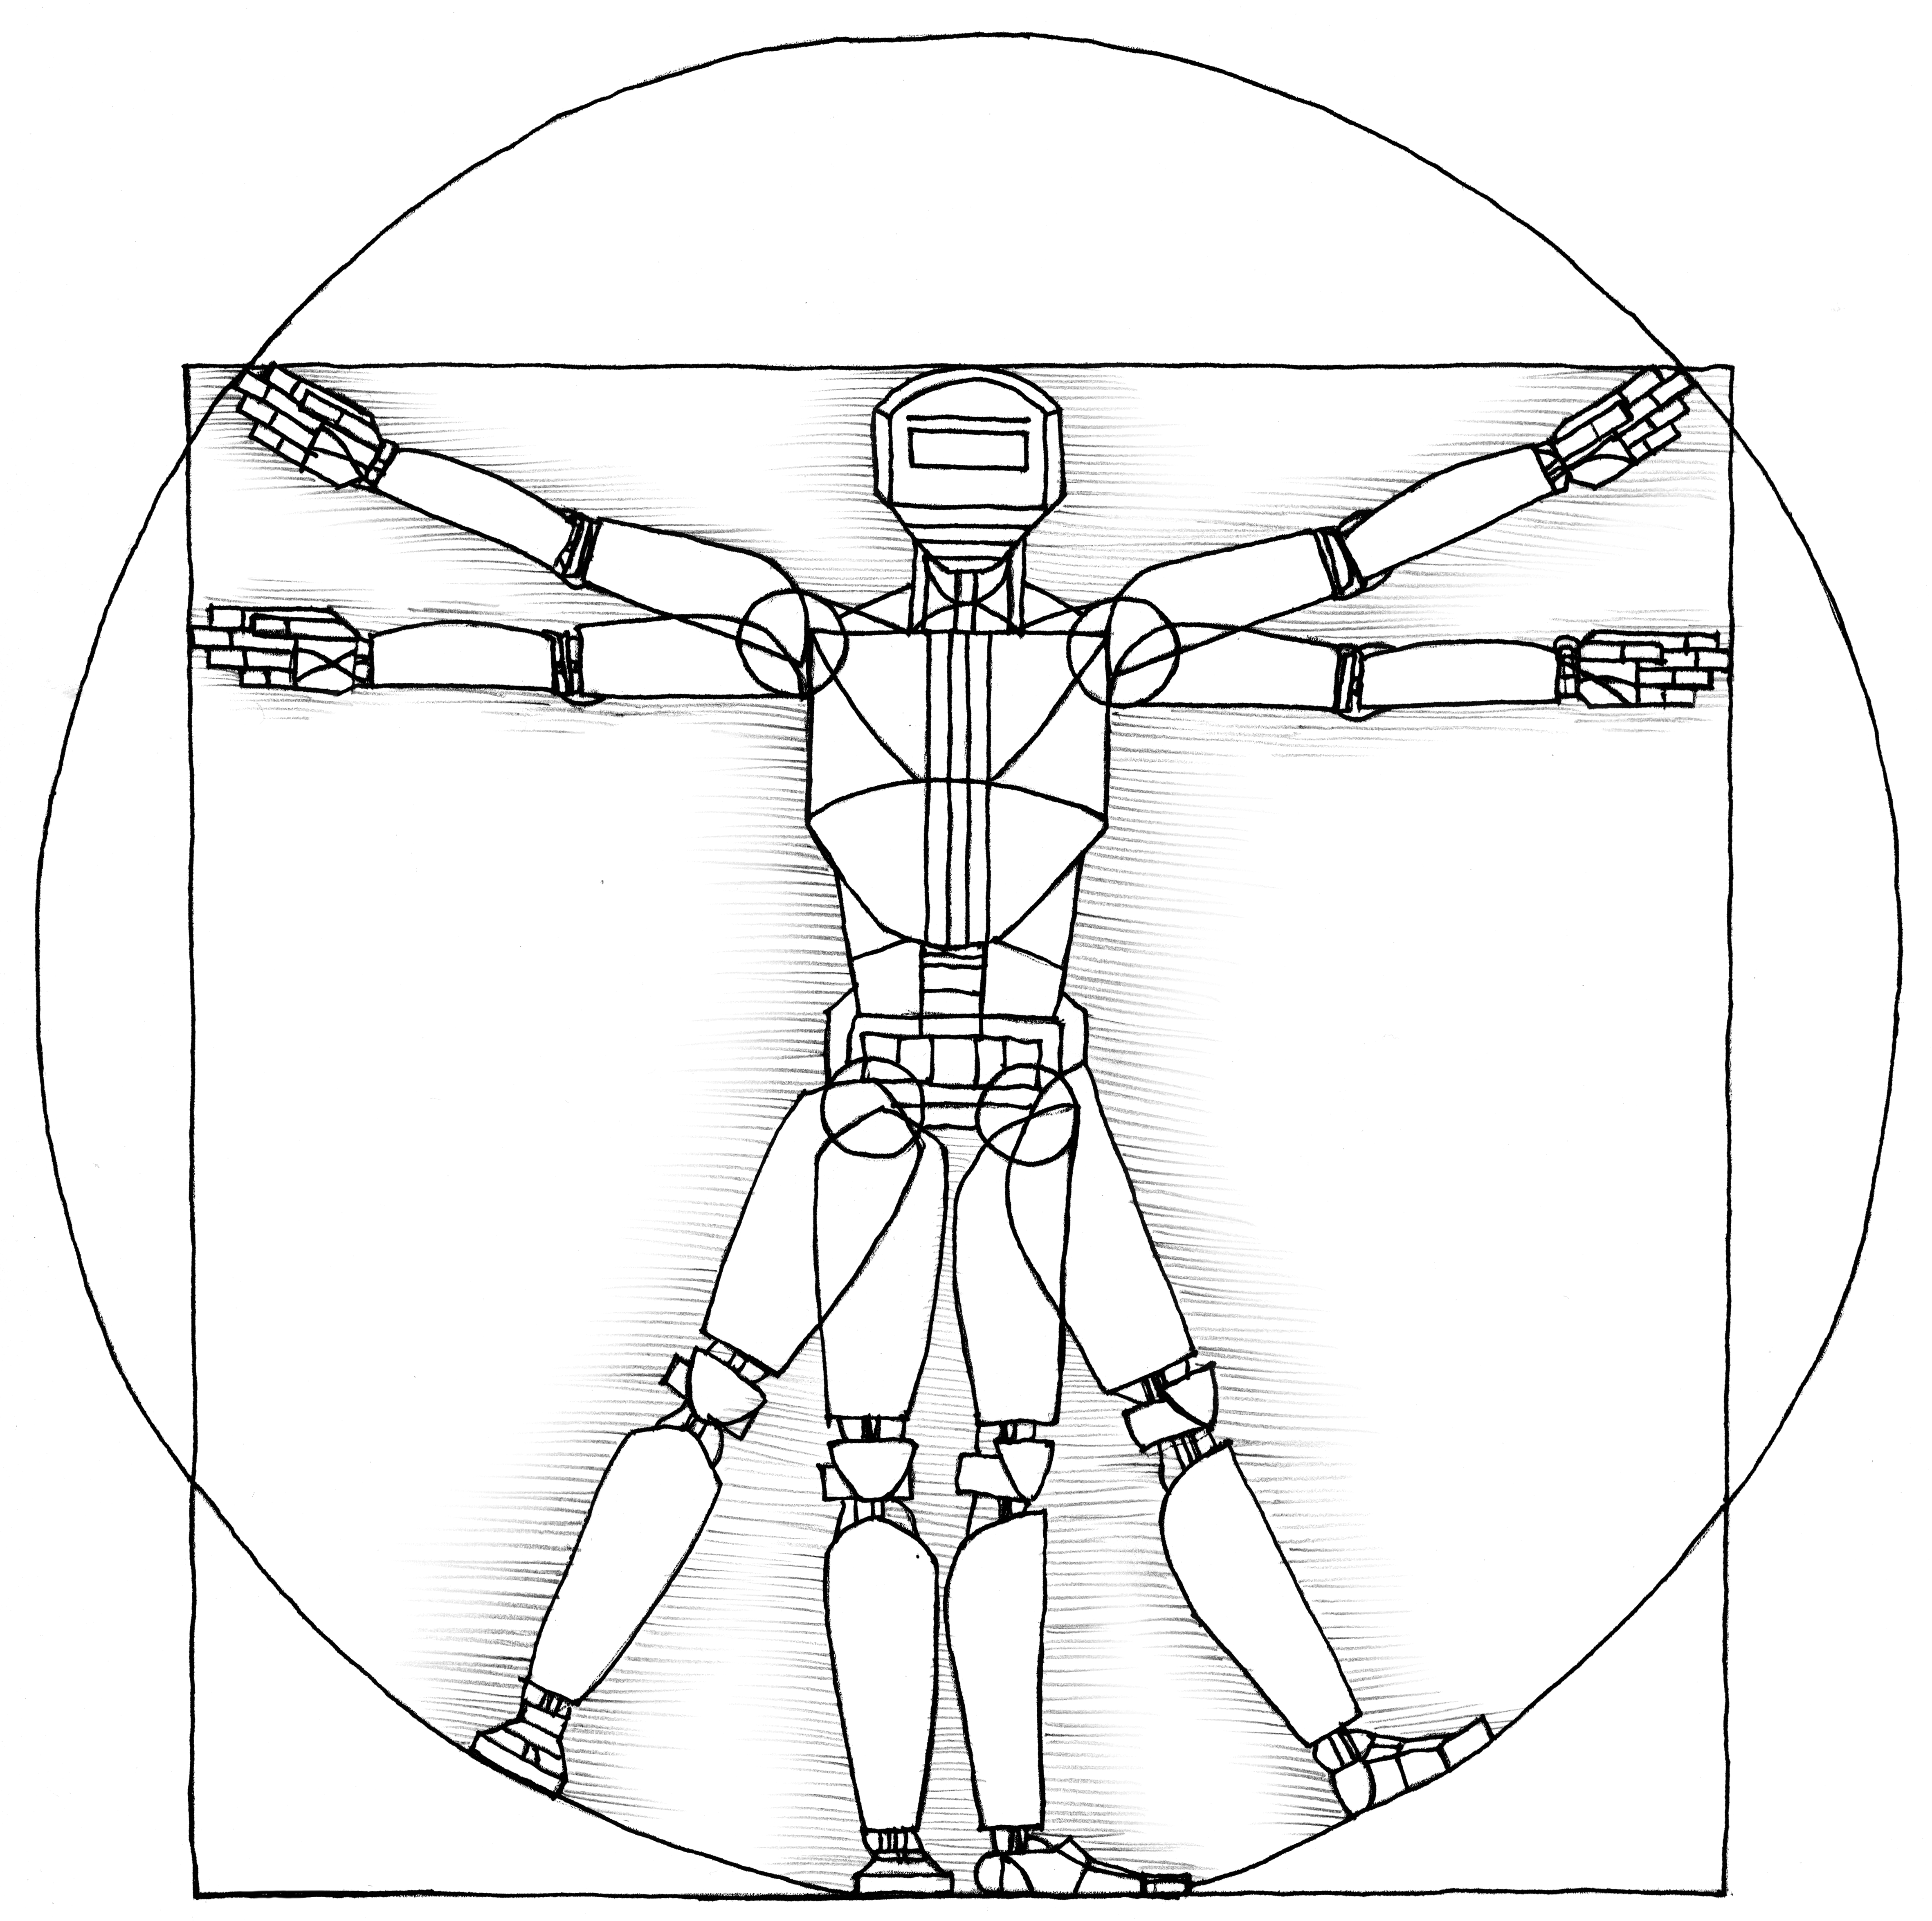
\includegraphics[width=15cm]{local_img/Robotics_Man}}

\begin{center}
{\Large Conference Booklet} \\[0.3cm]
       July 12--16, 2014 \\
       University of California, Berkeley\\
       Berkeley, California, USA\\
       www.roboticsconference.org
\end{center}
\clearpage
\pagestyle{front}



%%this puts the TOC on the same page as the preface
% \setcounter{tocdepth}{2}
% \begingroup
%   \let\clearpage\relax
%   %%%%%%%%%%%%%%%%%%%%%%%%%%%%%%%%%%%%%%%%%%%%%%%%%%%%

\chapter*{Preface}

%%%%%%%%%%%%%%%%%%%%%%%%%%%%%%%%%%%%%%%%%%%%%%%%%%%%

                                                                     
                                             
\vspace{3cm}
\section*{Welcome to RSS 2013!}
\begingroup{}
\Large
\vspace{1cm}

We welcome you to Robotics: Science and Systems 2013 at the Technische Universit\"at in the exciting city of Berlin!  We sincerely hope you will enjoy this week with exciting scientific contributions from all around the world in a city with an extraordinary and unique history.

Regarding this program booklet, we decided to go all electronic this year to be able to provide you with as much information as possible in a convenient manner. You can find schedules and detailed information online on the conference's homepage. We created a new mobile site for the \href{http://www.roboticsproceedings.org}{conference proceedings} of this and past RSS. In addition, we provide you with a USB stick that contains everything you need at the conference: from the daily schedules, venue maps, conference papers, and talk abstracts to lunch places and tips for evening activities.

\ifthenelse{\equal{\targetoutput}{print}}{     
   This booklet contains the basic information you will need for attendance, but we encourage you to use the electronic version!
}{
   This booklet and the links contained in it will be your central hub for information regarding conference papers, wireless network configuration, and many other things...
}

This year's RSS was made possible by many invisible hands that gave their support and put in long hours and hard work: the organizing committee, our sponsors, the area chairs, the many reviewers, workshop chairs, our resident graphic designer, the student volunteers, and so many more. Special thanks to everybody who contributed!

If we can help you with anything during the conference, please just contact us---we wear light blue T-shirts!  You can also always reach the registration desk at {\Large \textbf{ +49 163 697 6268} or +49 163 69-ROBOT}.  At the registration desk you will also find paper pads and pens, power adapters, Aspirin, lunch tips, transportation help, a boarding pass printer, and other useful things...

We hope you will actively participate in the scientific discourse throughout the coming days and will leave Berlin with new insights, memories of exciting discussions, inspiring talks, brilliant ideas as well as new collaborators and friends!


\vspace{1cm}

The Local Arrangements Committee


\endgroup{}
\normalsize

   %contains the preface page with the welcome
%   \vfill
%    \sf \tableofcontents
% \endgroup
% 

%%%%%%%%%%%%%%%%%%%%%%%%%%%%%%%%%%%%%%%%%%%%%%%%%%%%

\chapter*{Preface}

%%%%%%%%%%%%%%%%%%%%%%%%%%%%%%%%%%%%%%%%%%%%%%%%%%%%

                                                                     
                                             
\vspace{3cm}
\section*{Welcome to RSS 2013!}
\begingroup{}
\Large
\vspace{1cm}

We welcome you to Robotics: Science and Systems 2013 at the Technische Universit\"at in the exciting city of Berlin!  We sincerely hope you will enjoy this week with exciting scientific contributions from all around the world in a city with an extraordinary and unique history.

Regarding this program booklet, we decided to go all electronic this year to be able to provide you with as much information as possible in a convenient manner. You can find schedules and detailed information online on the conference's homepage. We created a new mobile site for the \href{http://www.roboticsproceedings.org}{conference proceedings} of this and past RSS. In addition, we provide you with a USB stick that contains everything you need at the conference: from the daily schedules, venue maps, conference papers, and talk abstracts to lunch places and tips for evening activities.

\ifthenelse{\equal{\targetoutput}{print}}{     
   This booklet contains the basic information you will need for attendance, but we encourage you to use the electronic version!
}{
   This booklet and the links contained in it will be your central hub for information regarding conference papers, wireless network configuration, and many other things...
}

This year's RSS was made possible by many invisible hands that gave their support and put in long hours and hard work: the organizing committee, our sponsors, the area chairs, the many reviewers, workshop chairs, our resident graphic designer, the student volunteers, and so many more. Special thanks to everybody who contributed!

If we can help you with anything during the conference, please just contact us---we wear light blue T-shirts!  You can also always reach the registration desk at {\Large \textbf{ +49 163 697 6268} or +49 163 69-ROBOT}.  At the registration desk you will also find paper pads and pens, power adapters, Aspirin, lunch tips, transportation help, a boarding pass printer, and other useful things...

We hope you will actively participate in the scientific discourse throughout the coming days and will leave Berlin with new insights, memories of exciting discussions, inspiring talks, brilliant ideas as well as new collaborators and friends!


\vspace{1cm}

The Local Arrangements Committee


\endgroup{}
\normalsize

   %contains the preface page with the welcome
\clearpage
\setcounter{tocdepth}{1}
\begingroup
  {\sf \small 
  \tableofcontents}
\endgroup

\clearpage
\pagestyle{default}

\chapter{Conference and Local Information}

\setlength\fboxsep{0pt}
\setlength\fboxrule{0.5pt}
%\phantomsection \section{Help and Emergencies}

%In case of an emergency at the conference, please call {\Large \textbf{911}}. You can also request help from any of the conference volunteers and the concierge at the main entrances of university buildings. For emergencies at the conference or elsewhere in USA, please call the emergency number {\Large \textbf{911}}. 

%If you need special assistance to access a building, please contact the registration desk at {\Large \textbf{NUMBER}}.

\vspace{-1.0cm}
\phantomsection \section{General Information}

\section*{About Berkeley}

Berkeley (pronounced burk-lee) is a city on the east shore of San Francisco Bay in northern Alameda County, California, that is named after the eighteenth-century bishop and philosopher George Berkeley. Berkeley borders the cities of Albany, Oakland, and Emeryville and Contra Costa County including unincorporated Kensington as well as San Francisco Bay. According to the United States Census Bureau the city's 17.7 square miles area includes 10.5 square miles of land and 7.2 square miles water, most of it part of San Francisco Bay. Its population at the 2010 census was determined to be 112,580 and it is one of the most politically liberal cities in the United States.

Berkeley is the site of the oldest campus in the University of California system – the University of California, Berkeley – and of the Lawrence Berkeley National Laboratory that the university manages and operates. 

Berkeley is served by Amtrak (Capitol Corridor), AC Transit, BART (Ashby, Downtown Berkeley Station and North Berkeley) and bus shuttles operated by major employers including UC Berkeley and Lawrence Berkeley National Laboratory. The Eastshore Freeway (Interstate 80 and Interstate 580) runs along the bay shoreline. Berkeley also hosts car sharing networks run by City CarShare, Uhaul Car Share, and Zipcar. Several "pods" (points of departure where cars are kept) exist throughout the city, in several downtown locations, at the Ashby and North Berkeley BART stations, and at various other locations in Berkeley (and other cities in the region).

Berkeley has a number of distinct neighborhoods. Surrounding the University of California campus are the most densely populated parts of the city. West of the campus is Downtown Berkeley, the city's traditional commercial core; home of the civic center, the city's only public high school, the busiest BART station in Berkeley, as well as a major transfer point for AC Transit buses. South of the campus is the Southside neighborhood, mainly a student ghetto, where much of the university's student housing is located. The busiest stretch of Telegraph Avenue is in this neighborhood. North of the campus is the quieter Northside neighborhood, the location of the Graduate Theological Union. North of Downtown is the North Berkeley neighborhood, which has been nicknamed the "Gourmet Ghetto" because of the concentration of well-known restaurants and other food-related businesses. In the southeastern corner of the city is the Claremont District, home to the Claremont Hotel; and the Elmwood District, with a small shopping area on College Avenue. West of Elmwood is South Berkeley, known for its weekend flea market at the Ashby Station. The areas of South and West Berkeley are in the midst of redevelopment. Along the shoreline of San Francisco Bay at the foot of University Avenue is the Berkeley Marina. 

\vspace{3mm}
\section*{About University of California, Berkeley}

The University of California, Berkeley (also referred to as UC Berkeley; Berkeley; California; or simply Cal), is a public research university located in Berkeley, California. The university occupies 1,232 acres (499 ha) on the eastern side of the San Francisco Bay with the central campus resting on 178 acres (72 ha). Berkeley is the flagship institution of the 10 campus University of California system.

Established in 1868 as the result of the merger of the private College of California and the public Agricultural, Mining, and Mechanical Arts College in Oakland, Berkeley is the oldest institution in the UC system and offers approximately 350 undergraduate and graduate degree programs in a wide range of disciplines. Berkeley has been charged with providing both "classical" and "practical" education for the state's people. Berkeley co-manages three United States Department of Energy National Laboratories, including the Los Alamos National Laboratory, Lawrence Livermore National Laboratory and Lawrence Berkeley National Laboratory for the U.S. Department of Energy.

%Berkeley faculty, alumni, and researchers have won 72 Nobel Prizes (including 30 alumni Nobel laureates), 9 Wolf Prizes, 7 Fields Medals, 15 Turing Awards, 45 MacArthur Fellowships, 20 Academy Awards, and 11 Pulitzer Prizes. 

\vspace{3mm}

\section*{Registration}

The registration desk will be located in the lobby of Wheeler Hall on the first floor. Student volunteers will be present at the desk and will provide you with a registration packet consisting of your name tag, wireless internet access credentials, a printed conference booklet, conference t-shirt, and tickets to the conference banquet and the Dinner \& Demos event at Google HQ.

\vspace{3mm}
\section*{Wireless Internet Access}
Conference participants will be able to access the campus-wide wireless \emph{AirBears} network. Access credentials are printed on your name tag. If you have difficulties setting up your wireless access, please contact any of the volunteers or the registration desk.

\vspace{3mm}
\section*{Help and Emergencies}
In case of an emergency at the conference, you can seek assistance from any of the conference volunteers (who will wear gold t-shirts) or seek assistance at the registration desk. For medical emergencies at the conference, please call 911.

\clearpage
\phantomsection \section{Conference and Workshops Venues}
%The following campus map shows the location.
\begin{figure}[h!]
\includegraphics[width=\linewidth]{local_img/maps/wheeler_hall}
\end{figure}

The conference, workshops, and interactive poster sessions will take place in Wheeler Hall on the UC Berkeley campus. 

\newpage
\phantomsection \section{1st Floor Plan of Wheeler Hall -- Conference Venue}
{\large Monday, July 14 to Wednesday, July 16}
\begin{figure}[h!]
\center
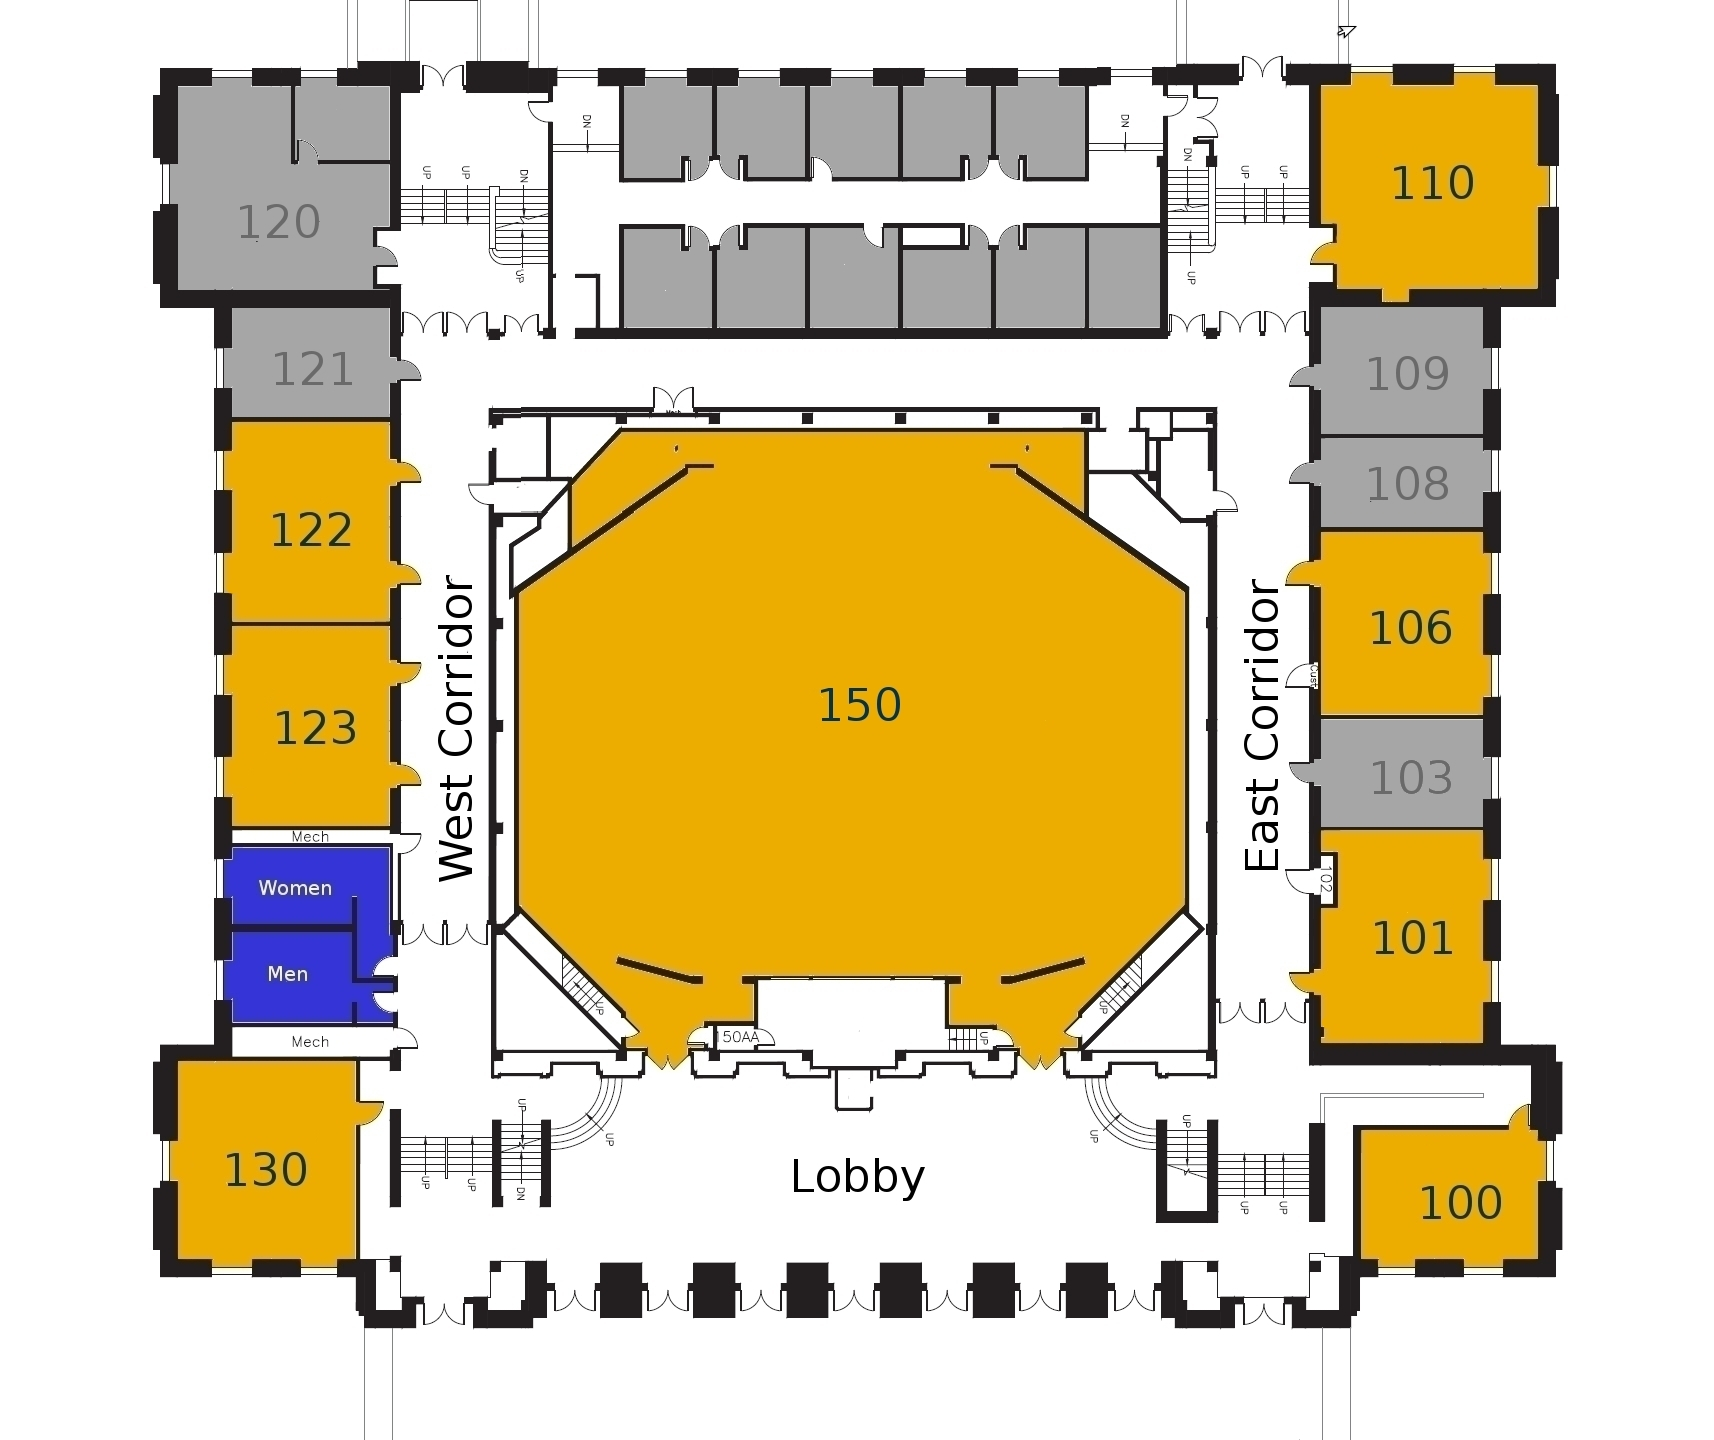
\includegraphics[height=0.6\textheight]{local_img/maps/first_floor}
\end{figure}

\newpage
\phantomsection \section{2nd Floor plan of Wheeler Hall -- Workshops Venue}
{\large Saturday, July 12 to Sunday, July 13}

\begin{figure}[h!]
\center
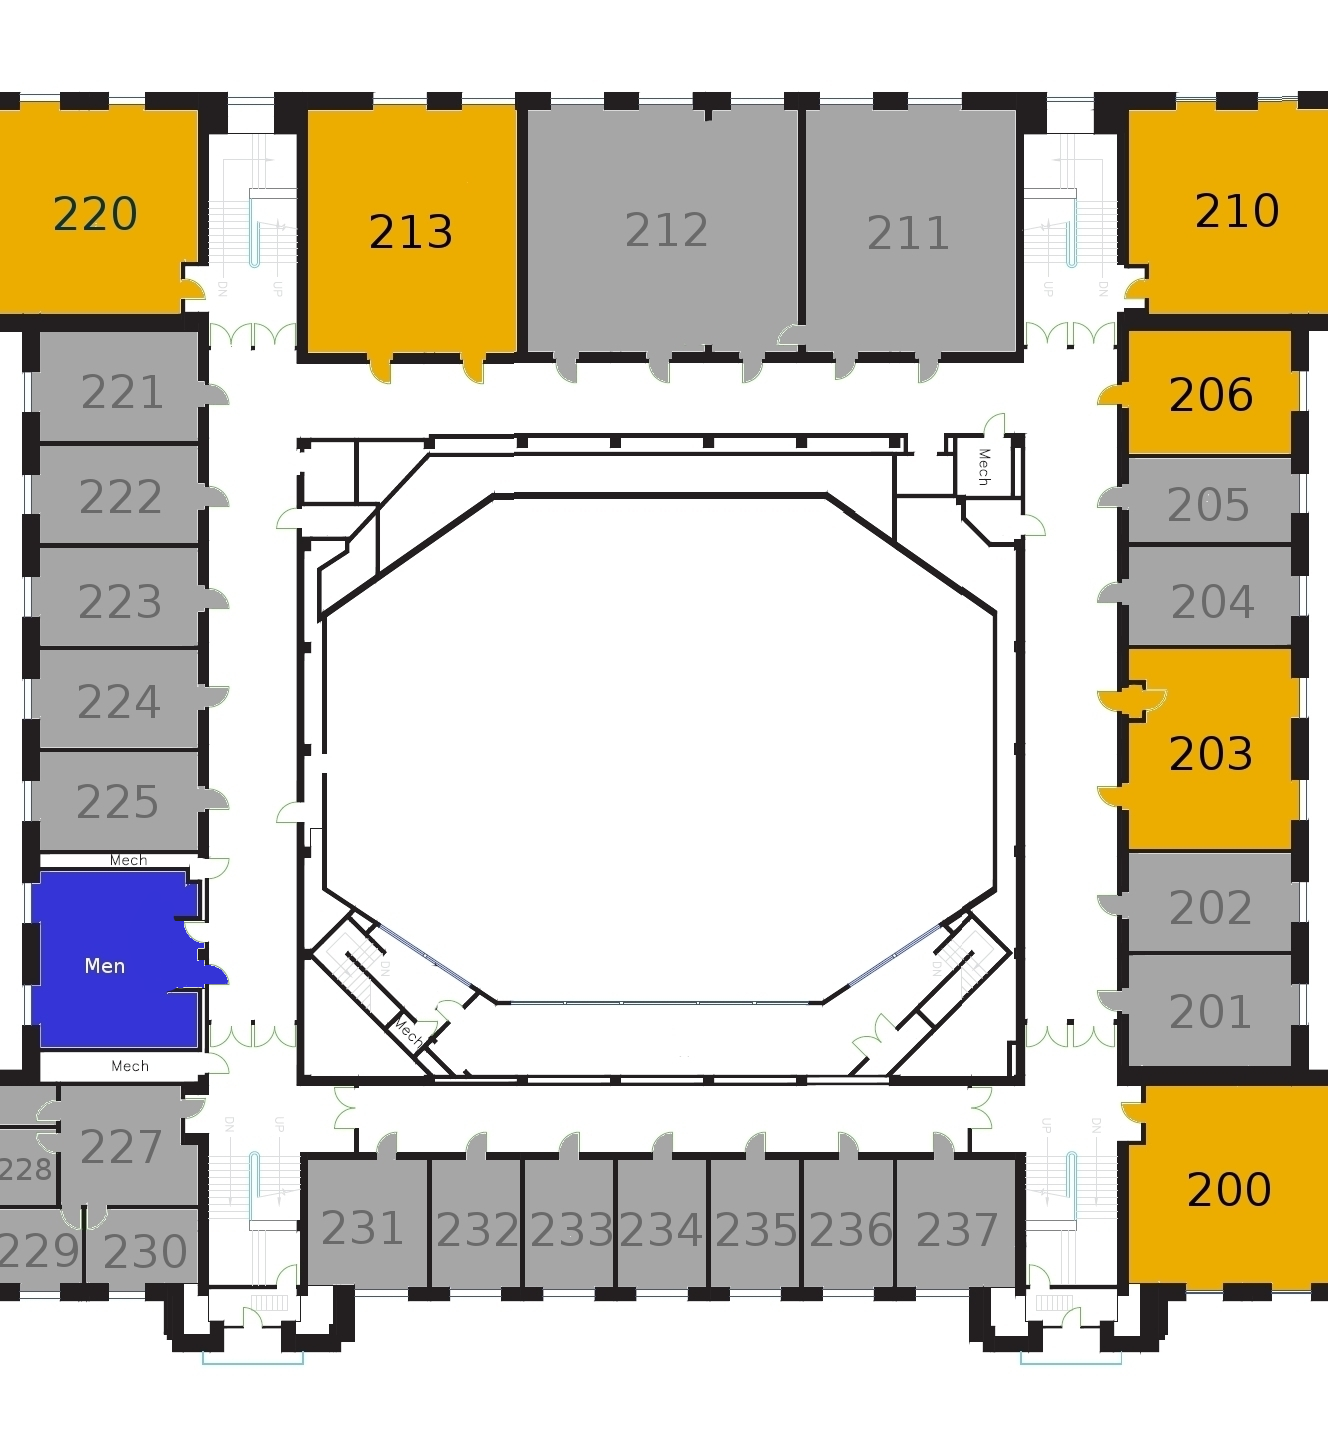
\includegraphics[height=0.6\textheight]{local_img/maps/second_floor}
\end{figure}

\clearpage

\phantomsection \section{Floor Plan Interactive Presentations}

\begin{figure}[h!]
\center
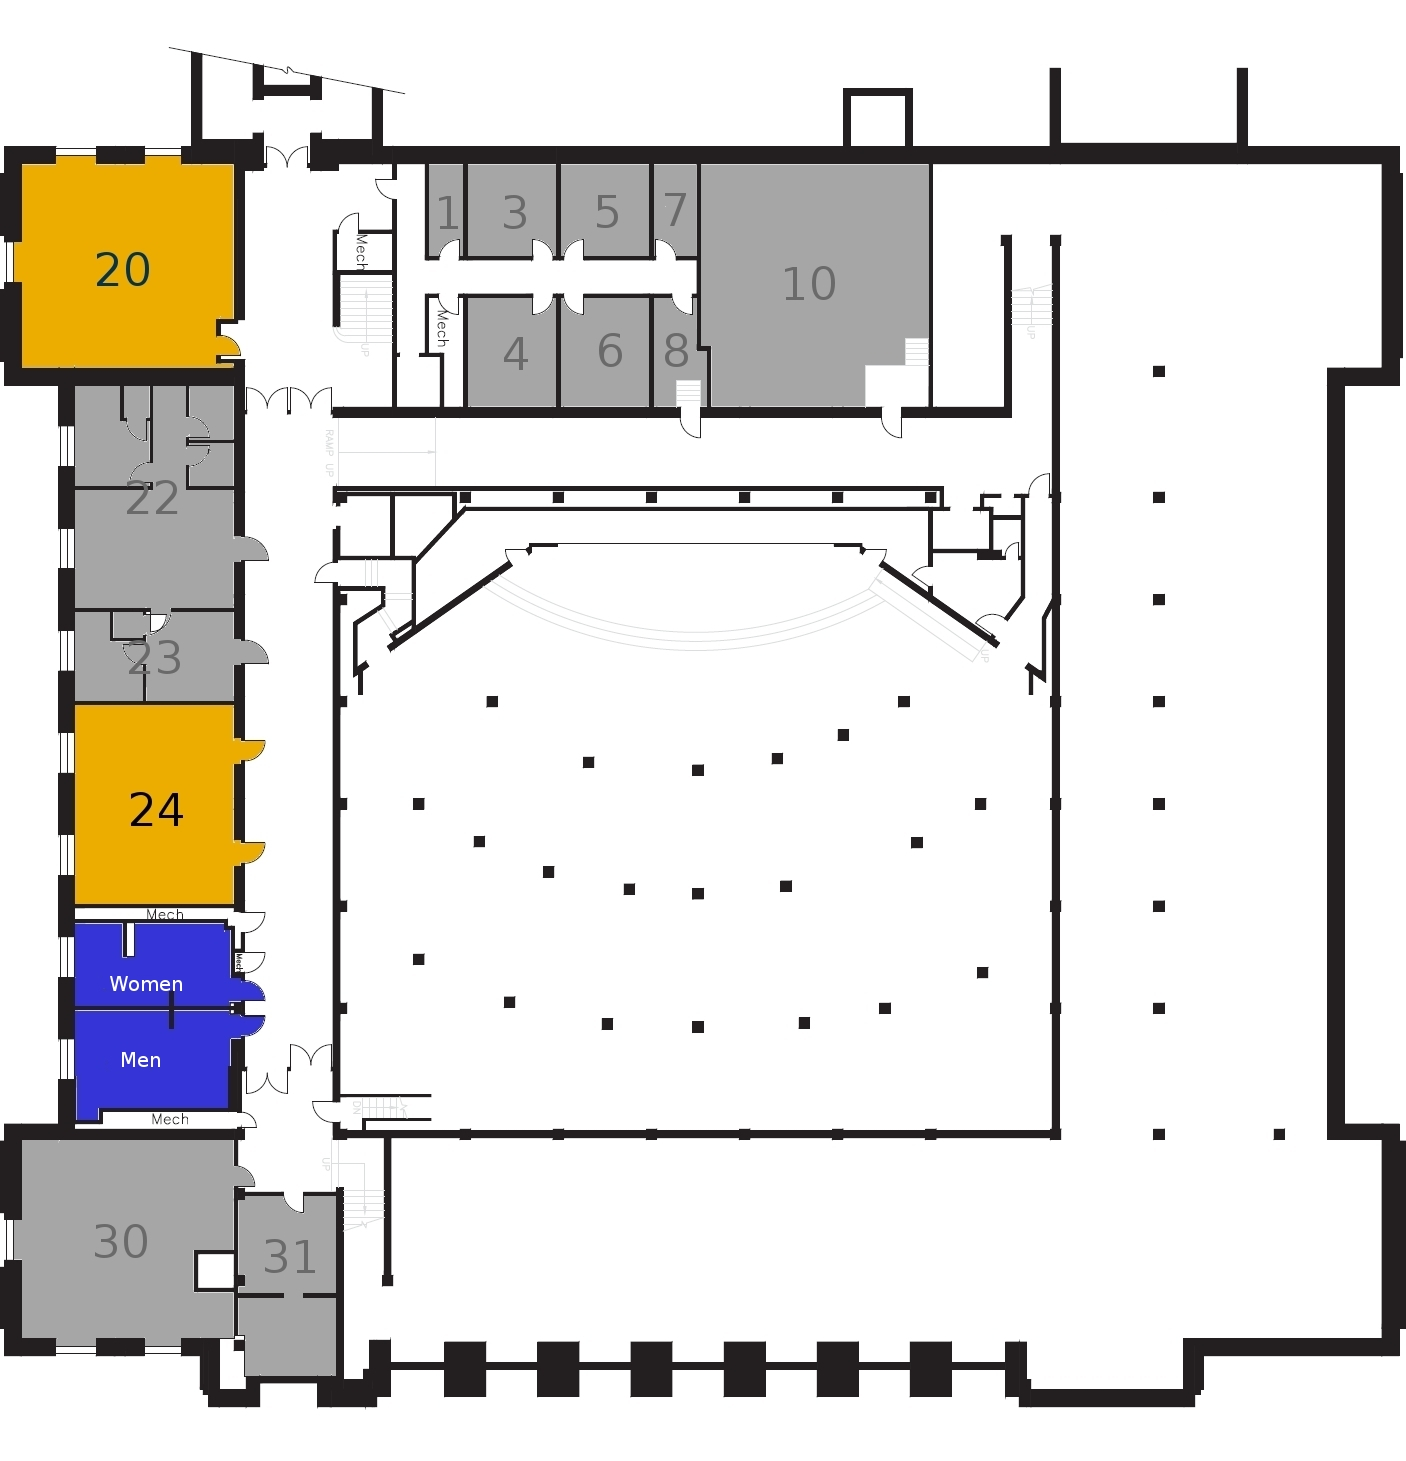
\includegraphics[height=0.6\textheight]{local_img/maps/basement}
\end{figure}


\phantomsection \section{Banquet Information}
The conference banquet will be held on a cruise on the San Francisco Bay. Enjoy a splendid sunset on the water with magnificent views of the city of San Francisco, accompanied by a
delicious seasonal dinner and drinks. Transportation will be provided. Buses will pick us up from Berkeley at 6pm and take us to Pier 3 in San Francisco, where we will board the San Francisco Belle. Buses will pick us up from Pier 3 around 10pm, and we'll be back in Berkeley
around 10:30pm.

%\label{sec:banquetinfo}
%\begin{figure}[h!]
%\center
%\fbox{\includegraphics[width=3in]{local_img/maps/katerholzig_labeled}}
%\end{figure}

%After crossing the bridge, turn left through a boarded fence and enter the venue via an unpaved path. When you start wondering whether you are at the right place, you are at the right place.  Just keep on walking.  The address of Kater Holzig is Michaelkirchstra{\ss}e 23; the GPS coordinates are: 52.511283,13.42393. 

%The trip takes about 45 minutes. The banquet will begin at 20:00.


%\begin{landscape}
%\phantomsection \section{Public transport map}
%\begin{figure}[h!]
%\includegraphics[height=0.9\textwidth, keepaspectratio]{local_img/maps/bvg}
%\end{figure}
%\end{landscape}


%set back fbox frame
\setlength\fboxrule{0pt}

    %contains sponsor information, about, general wuick info about arrangements

\chapter{Drink and Food Suggestions}

\setlength\fboxsep{0pt}
\setlength\fboxrule{0.5pt}

\vspace{-1.5cm}
\phantomsection \section{Lunch}

\begin{figure}[h!]
\center
\fbox{\includegraphics[width=6in]{local_img/maps/food.pdf}}
\end{figure}

We recommend the Southside, Northside, and Downtown neighborhoods for lunch in terms of proximity to the conference venue. We have provided below a sampling of lunch places in each of these neighborhoods, along with the type of food and price category. 

\vspace{1mm}

1) Southside (0.3 miles from Wheeler Hall)

\begingroup
\small
\begin{multicols}{1}[]
    \begin{tabular}{p{0.3cm} p{4cm} p{5cm} p{0.5cm}}
        1 & Cheese 'N' Stuff & Sandwiches & \$\\
        2 & Montague's Gourmet Sandwiches & Sandwiches & \$\\
        3 & Tivoli Caffe & Pizza, Sandwiches & \$\\
        4 & Gypsy's Trattoria Italiano & Italian  & \$\\
        5 & Julie's Cafe & Sandwiches, Salads & \$\\ 
        6 & KoJa Kitchen & Asian Fusion, Japanese & \$\\
        7 & Crepes A-Go Go & Creperie & \$\\
        8 & Chipotle Mexican Grill & Mexican & \$\\
        9 & Free House & Burgers, Salads, Sandwiches & \$\$\\
        10 & Henry's & Burgers, Salads, Sandwiches & \$\$\\
    \end{tabular}
\end{multicols}
\endgroup
\normalsize 

2) Northside (0.5 miles from Wheeler Hall)

\begingroup
\small
\begin{multicols}{1}[]
    \begin{tabular}{p{0.3cm} p{4cm} p{5cm} p{0.5cm}}
        1 & Northside Cafe & Breakfast, Sandwiches & \$\\
        2 & Urbann Turbann & Rice/Naan Wraps with Indian Curries & \$\\
        3 & D'Yar & Mediterranean & \$\\
        4 & The Pho Bar & Vietnamese  & \$\$\\
        5 & Cafe Nefeli & Mediterranean & \$\\ 
        6 & Bongo Burger & Burgers, Salads & \$\\
        7 & Celia's Mexican & Mexican & \$\$\\
        8 & Stuffed Inn & Sandwiches & \$\\
        9 & Jasmine Thai & Thai & \$\$\\
        10 & Hummingbird Cafe & Sandwiches, Mediterranean & \$\\
    \end{tabular}
\end{multicols}
\endgroup
\normalsize 

3) Downtown (1 mile from Wheeler Hall)

\begingroup
\small
\begin{multicols}{1}[]
    \begin{tabular}{p{0.3cm} p{4cm} p{5cm} p{0.5cm}}
        1 & Slow & Sandwiches & \$\\
        2 & Platano & Latin American & \$\$\\
        3 & Brazil Cafe & Brazilian, Sandwiches & \$\\
        4 & PIQ Bakery & Italian, Bakery  & \$\\
        5 & Sandwich Spot & Sandwiches & \$\\ 
        6 & Gecko Gecko & Thai & \$\$\\
        7 & Athineon & Mediterranean & \$\$\\
        8 & Sliver & Pizza, Sandwiches & \$\\
        9 & Toss Noodle Bar & Asian Fusion & \$\\
        10 & Suya African Caribbean Grill & African, Caribbean & \$\\
    \end{tabular}
\end{multicols}
\endgroup
\normalsize 

\phantomsection \section{Dinner}

There are a plethora of dining options available in the Berkeley neighborhoods listed on the map. We have provided below a sampling of dinner places that we like. This list is by no means comprehensive and we encourage you to check out dining options on Yelp! or Google maps as well. We recommend that you reserve a table in advance, especially on Saturday and Sunday.

\begingroup
\small
\begin{multicols}{1}[]
    \begin{tabular}{p{0.3cm} p{4cm} p{5cm} p{1cm} p{2cm}}
        1 & Gather & American, Drinks & \$\$ & Downtown \\
        2 & Jupiter & America, Drinks, Brewery & \$\$ & Downtown \\
	    3 & Comal & Mexican, Drinks & \$\$ & Downtown \\       
	    4 & Five & American, Drinks & \$\$\$ & Downtown \\ 
        5 & Cesar & Tapas Bar & \$\$\$ & Gourmet Ghetto\\
        6 & Cheese Board & Pizza & \$ & Gourmet Ghetto \\
        7 & Cha-Am & Thai & \$\$ & Gourmet Ghetto\\
        8 & Chez Panisse & French & \$\$\$\$ & Gourmet Ghetto \\
        9 & Taste of the Himalayas & Indian, Nepalese & \$\$ & Gourmet Ghetto \\
        10 & Henry's & American, Drinks & \$\$ & Southside \\
        11 & Free House & American, Drinks & \$\$ & Southside \\
        12 & Kiraku & Japanese Tapas & \$\$ & Southside \\
        13 & Wood Tavern & American, Drinks & \$\$\$ & Elmwood \\
        14 & Rangoon Super Stars & Burmese & \$\$ & Elmwood\\
        15 & Ici & Ice-cream & \$ & Elmwood\\
    \end{tabular}
\end{multicols}
\endgroup
\normalsize 

\setlength\fboxrule{0pt}
    %contains maps, event lists, and lunch/dinner/bar guides

%%%%%%%%%%%%%%%%%%%%%%%%%%%%%%%%%%%%%%%%%%%%%%%%%%%%

\chapter{Invited Talks}

%%%%%%%%%%%%%%%%%%%%%%%%%%%%%%%%%%%%%%%%%%%%%%%%%%%%
%some helper commands for common formatting:
\newcommand{\invitedTalk}[7]{
 \begin{minipage}[t]{0.48\textwidth}
 \vspace{1em}
 \begingroup
  \sf
  {\Large #4\\}
  {\LARGE #1\\}
  \begin{spacing}{1.0}

     {\LARGE \raggedright #2}
     
  \end{spacing}
  %\vspace{5mm}
  \endgroup
  \normalsize
  #6
  
 \end{minipage}
 ~\hfill~
 \begin{minipage}[t]{0.43\textwidth}
  \begin{flushright}
   \vspace{1em}
     \ifthenelse { \equal{#5}{} } {
	%\vspace{2cm}
     } {
              \includegraphics[height=5cm]{local_img/speakers/#5}\\
     }
     \textbf{#1}\\
     #3 \\[5mm]
  \end{flushright}
  {\small \textbf{Biography}
  
  #7
  
  }
\end{minipage}
\vspace{1cm}
%\clearpage

}


\vspace{-2cm}
%%%%%%%%%%%%%%%%%%%%%%%%%%%%%%%%%%%%%%%%%%%%%%%%%%%%
\invitedTalk{Chris Urmson}{Realizing Self-Driving Cars}{Google [x]}{Monday, July 14, 09:00}{urmson.jpg}
{
Self-driving vehicles are coming. They will save lives, save time and offer mobility to those who otherwise don't have it. Eventually they will reshape the way we live in, and move through, our communities and cities. Or so the story goes. Is this a 50 year pipe dream, or a near term reality? A dedicated team at Google has spent the last five years moving self-driving vehicles closer to a reality. New algorithms, increased processing power, innovative sensors and massive amounts of data enable our vehicles to see further, understand more and handle a wide variety of challenging driving scenarios. Our vehicles have driven over a half million miles on highways, suburban and urban streets. Through this journey, we've learned a lot; not just about how to drive, but about interacting with drivers, users and others on the road, and about what it takes to bring in incredibly complex system to fruition. I'll share some fun stories and lessons along with our vision for how these vehicles will become a reality.
}{
Chris Urmson leads Google's self-driving car program where the team's vehicles have driven over a half million miles. Prior to joining Google, Chris was on the faculty of the Robotics Institute at Carnegie Mellon University where his research focused on motion planning and perception for robotic vehicles. During his time at Carnegie Mellon, he worked with house size trucks, drove robots around in deserts and served as the Director of Technology for the team that won the 2007 DARPA Urban Challenge. He earned his PhD in 2005 from Carnegie Mellon and his B.Sc. in Computer Engineering from the University of Manitoba in 1998.
}





%%%%%%%%%%%%%%%%%%%%%%%%%%%%%%%%%%%%%%%%%%%%%%%%%%%%
\invitedTalk{Genevieve Bell}{The Pre-history of Robots}{Intel}{Monday, July 14, 14:00}{bell.jpg}
{
Genevieve Bell is a well known anthropologist, working at the intersection of culture and technology. Australian by birth, Bell runs one of Intel's premier research and development labs in the United States. In this talk, she unpacks the relationship between technology and anxiety, tracing out the origins of our socio-technical fears. Drawing on cultural, literary and historical accounts, Bell makes the case that we have an opportunity to re-imagine the ways in which we encounter and make sense of new digital technologies.
}{
Dr. Genevieve Bell is an anthropologist and researcher with 15 years of experience driving innovation in the high tech industry. As the Director of Interaction and Experience Research in Intel Labs, Bell leads a team of social scientists, interaction designers, human factors engineers and computer scientists. This organization researches new computing experiences that are centered around people's needs and desires. This foundationally shapes and then helps to create new Intel technologies and products. In this team and her prior roles, Bell has fundamentally altered the way Intel envisions and plans its products so that they are centered on people's needs rather than simply silicon capabilities. In addition to leading this increasingly important area at Intel, Bell is an accomplished industry commentator on the intersection of culture and technology and has been extensively featured in publications that include Wired, Forbes, The Atlantic, Fast Company, and the Wall Street Journal. In August 2013, Fast Company declared her to be one of the top 25 smartest women on Twitter, where she goes by the handle, @feraldata. She is a regular public speaker and panelist at technology conferences worldwide, sharing myriad insights gained from her extensive international field work and research. In 2010, Bell was named one of Fast Company's inaugural '100 Most Creative People in Business.' Bell is a passionate advocate for the advancement of women in technology and in 2012 was inducted into the Women In Technology International (WITI) hall of fame, as well being honored by the Anita Borg Institute as the 2013 Woman of Vision for Leadership. Her first book, 'Divining the Digital Future: Mess and Mythology in Ubiquitous Computing,' was co-written with Prof. Paul Dourish of the University of California at Irvine and released in April 2011. Bell is also the recipient of several patents for consumer electronics innovations. A native of Australia, Bell moved to the United States for her undergraduate studies and graduated from Bryn Mawr in 1990 with a bachelor's degree in anthropology. She then earned a master's degree and a doctorate in cultural anthropology from Stanford University where she also taught as an acting lecturer in the Department of Anthropology from 1996-1998. With a father who was an engineer and a mother who was an anthropologist, perhaps Bell was fated to ultimately work for a technology company, joining Intel in 1998. Bell is currently an Intel Fellow.
}



%%%%%%%%%%%%%%%%%%%%%%%%%%%%%%%%%%%%%%%%%%%%%%%%%%%%
\invitedTalk{Brad Nelson}{Swimming Microrobots}{ETH Zurich}{Tuesday, July 15, 09:00}{nelson.jpg}
{
Nature has inspired numerous microrobotic locomotion designs that are suitable for propulsion generation at low Reynolds numbers. This talk first reviews various swimming methods with a particular focus on helical propulsion inspired by E. coli bacteria. To actuate swimming microrobots, various magnetic actuation methods have been proposed, such as rotating fields, oscillating fields, and field gradients. These methods can be categorized into force-driven or torque-driven actuation. It can be shown that torque-driven approaches scale better to the micro- and nano-scale than force-driven approaches. The implementation of swarm or multi-agent control will also be discussed. The use of multiple microrobots may be beneficial for in vivo as well as in vitro applications, and the frequency-dependent behavior of helical microrobots allows individual agents to be decoupled from within small groups. Finally, an elegant commercial application of microrobots originally inspired by helical swimmers will be presented.
}{
Brad Nelson is the Professor of Robotics and Intelligent Systems at ETH Zurich. His primary research focus is on microrobotics and nanorobotics emphasizing applications in biology and medicine. He received mechanical engineering degrees from the University of Illinois (B.S. 1984) and the University of Minnesota (M.S. 1987) and a Ph.D. in Robotics (School of Computer Science) from Carnegie Mellon University (1995). He has worked as an engineer at Honeywell and Motorola and served as a United States Peace Corps Volunteer in Botswana, Africa. He was an Assistant Professor at the University of Illinois at Chicago (1995-1998) and an Associate Professor at the University of Minnesota (1998-2002). He became a Full Professor at ETH Zurich in 2002. Prof. Nelson has received a number of awards including more than a dozen Best Paper Awards at major robotics conferences and journals. He was named to the 2005 "Scientific American 50," Scientific American magazine's annual list recognizing fifty outstanding acts of leadership in science and technology from the past year for his efforts in nanotube manufacturing. His laboratory won the 2007 and 2009 RoboCup Nanogram Competition, both times the event has been held. He is a European Research Council Advanced Grantee (2011) and his lab appears in the 2012 Guinness Book of World Records for the "Most Advanced Mini Robot for Medical Use." In 2013 he was listed as an ISI Highly Cited Researcher. He serves on the editorial boards of several journals, has chaired several international workshops and conferences, has served as the head of the ETH Department of Mechanical and Process Engineering, the Chairman of the ETH Electron Microscopy Center (EMEZ), and is a member of the Research Council of the Swiss National Science Foundation.
}


%%%%%%%%%%%%%%%%%%%%%%%%%%%%%%%%%%%%%%%%%%%%%%%%%%%%
\invitedTalk{Andrew Ng}{Deep Learning: Machine Learning via Large-scale Brain Simulations}{Stanford University}{Wednesday, July 16, 09:00}{ng.jpg}
{
Machine learning is a very successful technology, but applying it to a new problem usually means spending a long time hand designing the input features to feed to the learning algorithm. This is true for applications in vision, audio, and text/NLP. To address this, researchers in machine learning have recently developed "deep learning" algorithms, which can automatically learn feature representations from unlabeled data, thus bypassing most of this time-consuming engineering. These algorithms are based on building massive artificial neural networks that were loosely inspired by cortical (brain) computations. In this talk, I describe the key ideas behind deep learning, and also discuss the computational challenges of getting these algorithms to work. I'll also present a few case studies, and report on the results from a project that I led at Google to build massive deep learning algorithms, resulting in a highly distributed neural network trained on 16,000 CPU cores, and that learned by itself to discover high level concepts such as common objects in video.
}{
Andrew Ng's research is in the areas of machine learning and artificial intelligence. Through building very large-scale cortical (brain) simulations, he is developing algorithms that can learn to sense and perceive without needing to be explicitly programed. Using these techniques, he has developed sophisticated computer vision algorithms, as well as a variety of highly capable robots, such as by far the most advanced autonomous helicopter controller, that is able to fly spectacular aerobatic maneuvers. His group at Stanford University (together with Willow Garage) also developed ROS, which is today by far the most widely used open-source robotics software platform. In 2011, he taught an online Machine Learning class to over 100,000 students, leading to the founding of Coursera, which is today the world's largest MOOC platform. Ng has also been named to the 2013 "Time 100" list of the most influential people in the world.
}

%%%%%%%%%%%%%%%%%%%%%%%%%%%%%%%%%%%%%%%%%%%%%%%%%%%%
\invitedTalk{Nancy Amato}{Using Motion Planning to Study Protein Motions}{Texas A\&M University}{Wednesday, July 16, 14:00}{amato.jpg}
{
Protein motions, ranging from molecular flexibility to large-scale conformational change, play an essential role in many biochemical processes. For example, some devastating diseases such as Alzheimer's and bovine spongiform encephalopathy (Mad Cow) are associated with the misfolding of proteins. Despite the explosion of structural and functional data, our understanding of protein movement is still very limited because it is difficult to measure experimentally and computationally expensive to simulate. In this talk, we describe how techniques developed for motion planning in robotics have been adapted and applied to model and analyze protein motions and to reason about the structure, flexibility and interactions of proteins and other biomolecules. These techniques adapt sampling-based methods developed for robotic configuration spaces to construct approximate maps of a protein's potential energy landscape which can be used, e.g., to generate transitional motions of a protein to the native state from unstructured conformations or between specified conformations. For example, we show how our map-based tools for modeling and analyzing folding landscapes can capture subtle folding differences between protein G and its mutants, NuG1 and NuG2.
}{
Nancy M. Amato is Unocal Professor and Interim Department Head of the Department of Computer Science and Engineering at Texas A\&M University where she co-directs the Parasol Lab. She received undergraduate degrees in Mathematical Sciences and Economics from Stanford University, and M.S. and Ph.D. degrees in Computer Science from UC Berkeley and the University of Illinois at Urbana-Champaign. Her main areas of research focus are motion planning and robotics, computational biology and geometry, and parallel and distributed computing. She was Editor-in-Chief of the IEEE/RSJ IROS Conference Paper Review Board from 2011-2013, has served on the editorial boards of the IEEE Transactions of Robotics and Automation, IEEE Transactions on Parallel and Distributed Computing, and is an elected member of the Administrative Committee of the IEEE Robotics and Automation Society. She was co-Chair of the NCWIT Academic Alliance (2009-2011), is a member of the Computing Research Association's Committee on the Status of Women in Computing Research (CRA-W) and of the Coalition to Diversity Computing (CDC). She was an AT\&T Bell Laboratories PhD Scholar, received an NSF CAREER Award, is a Distinguished Speaker for the ACM Distinguished Speakers Program, and was a Distinguished Lecturer for the IEEE Robotics and Automation Society. She received the 2013 IEEE Hewlett-Packard/Harriet B. Rigas Award, and a University-level teaching award and the Betty M. Unterberger Award for Outstanding Service to Honors Education at Texas A\&M. She is a AAAS Fellow and an IEEE Fellow.
}


\chapter{Early Career Spotlight}

\invitedTalk{Siddhartha Srinivasa}{The Mathematics of Human Robot Interaction}{Carnegie Mellon University}{Monday, June 24, 15:30}{srinivasa.jpg}
{
For years, the focus of robot motion planning has been to produce functional motion: industrial robots move to weld parts, vacuuming robots move to suck dust, and personal robots move to clean up a dirty table. We have been exploring the thesis that although functional motion is ideal when robots perform tasks in isolation, it is insufficient for collaboration, where a human and a robot are manipulating in a tightly-coupled shared workspace. Our goal is to make this collaboration fluent and seamless. To this end, we have been developing algorithms where the notion of an observer watching the motion is woven into the fabric of the motion planner. This perspective has allowed us to formalize qualitative notions such as predictability and legibility in psychology in terms of Bayesian inference and inverse optimal control, and to develop generative models for such motion using functional gradient optimization. I will also describe some of our user studies on applying these algorithms to human-robot handovers, 
assistive teleoperation, and shared workspace collaboration, and ongoing work on deception, ambiguity, and emotive motion.
}{
Siddhartha Srinivasa is an Associate Professor at the Robotics Institute at Carnegie Mellon University. His research focuses on manipulation, with the goal of enabling robots to robustly and gracefully interact with the world to perform complex manipulation tasks in uncertain, unstructured, and cluttered environments. His current research focuses on physics-based nonprehensile manipulation for reconfiguring clutter, functional gradient methods for motion planning, and formalizing HRI principles using machine learning, motion planning and optimization algorithms. Sidd is a recipient of the HRI Best Paper Award (2010), ONR Young Investigator Award (2012), Okawa Research Award (2012), and a best-paper finalist at RSS (2012, 2013), IEEE ICRA (2009, 2010, 2012), IEEE IROS (2010), and RO-MAN (2012). Sidd also captains the CMU squash team, and dreams of running ultra-marathons.
}


\invitedTalk{Hadas Kress-Gazit}{High-Level Verifiable Robotics}{Cornell University}{Monday, June 24, 16:30}{kress-gazit.jpg}
{
Why don’t we have robots fetching us coffee and finding our keys for us? While robots have become more capable and powerful, they are not yet integrated into everyday life. Part of the reason for this is that robots are difficult to program and even more difficult to verify. Therefore, to achieve the dream of a robot in every home, two key challenges must be addressed; people should be able to easily interact with robots, and robots must always do as they are told.

In this talk I will discuss the work done in my group to address these challenges. Specifically, I will describe the use of language and temporal logic to capture high-level task specifications and the development of formal methods that take the task specifications and produce correct robot behavior, if such behavior exists.
}{
Hadas Kress-Gazit is an Assistant Professor at the Sibley School of Mechanical and Aerospace Engineering at Cornell University. She received her Ph.D. in Electrical and Systems Engineering from the University of Pennsylvania in 2008 and has been at Cornell since 2009. Her research focuses on formal methods for robotics and automation and more specifically on creating verifiable robot controllers for complex high-level tasks using logic, verification, synthesis, hybrid systems theory and computational linguistics. She received an NSF CAREER award in 2010 and a DARPA Young Faculty Award in 2012.
}
 %abstracts of invited talks

\chapter{Workshops on Thursday, June 27}
\begin{spacing}{1.0}

%\descriptionWorkshop{ID}{room}{title}{online link}{abstract}{timetable}

\newcommand{\descriptionWorkshop}[5]{
\begingroup{}
\vspace{8mm}
  \section*{{\huge \textbf{#1}} #3}  

%whether to add link or not::
\ifthenelse{\equal{\targetoutput}{print}}{
  \ifthenelse{\equal{#4}{}}{
  
  }{
      workshop homepage\footnote{\url{#4}} 
  }
  \hfill {\bf {\large #2} }
}{
  \href{#4}{workshop homepage}
  \hfill {\bf #2 }
}
\\*
{#5}
\endgroup{}
}


\newcommand{\descriptionLabTour}[5]{
\begingroup{}
\vspace{8mm}
  \section*{{\huge \textbf{#1}} #3}  

%whether to add link or not::
\ifthenelse{\equal{\targetoutput}{print}}{
  \ifthenelse{\equal{#4}{}}{
  
  }{
      Lab homepage\footnote{\url{#4}} 
  }
  \hfill {\bf {\large #2} }
}{
  \href{#4}{Lab homepage}
  \hfill {\bf #2 }
}
\\*
{#5}
\endgroup{}
}



\vspace*{-2.0cm}

\descriptionWorkshop{01}{Thursday Morning, MAR 4.063}{Aerial Mobile Manipulation}{http://mysite.du.edu/~rvoyles/RSSwebsite.pdf}
{
The Osprey, a magnificent bird of prey that dives from undetectable heights to snatch fish from the water with its agile talons, is a master of aerial mobile manipulation. But the "snatch-and-go" is not representative of dexterous manipulation. The octopus, on the other hand, is one of the few known animals that manipulates while locomoting and does so while "flying" with great agility. Aerial mobile manipulation is a growing area of robotics research that endeavors to become the "octopus of the air" while starting out as an osprey. Capitalizing on the ubiquity of low cost and easy to fly UAVs, great strides have been made in a short time. A natural extension of the rebirth of interest in manipulation represented by the mobile manipulation community, aerial mobile manipulation addresses new challenges and overcomes new constraints not familiar to UGVs. But aerial mobile manipulation is still manipulation at heart, and manipulation requires careful attention to dynamics and collaboration which are sometimes overlooked in the practical process of defying gravity and mastering the snatch-and-go. This workshop proposes to bridge the theoretical and experimental by bringing together manipulation experts, UAV experts, real-time perception experts, and collaboration experts to present and discuss the current and future of aerial mobile manipulation.
}

\descriptionWorkshop{02}{Thursday Morning, MAR 0.003}{Sensitive Robotics}{http://users.wpi.edu/~etorresj/RSSSensitiveRobotics/}
{
New sensing technologies are allowing robots to be more aware of the interaction between their body and their environment. Such is the case for tactile sensors in arms and hands, MEMS air sensors in flying robots, and MEMS flow sensors in swimming robots. Processing these types of sensory input poses new challenges such as: modeling for large array of sensors, dealing with sparse information, representing sensor in reconfigurable structures like arms or wings. This workshop intends to bring people together from different areas of robotics that work with large
arrays of sensors based on direct contact rather than light or other radiation, to discuss their different approaches.
}




\descriptionWorkshop{03}{Thursday, MAR 0.010}{Common Platforms in Robotic Manipulation}{http://www.willowgarage.com/coman13}
{
This workshop will focus on common hardware and software platforms for robotic manipulation. Participants will present work related to this theme, including open source hardware, software and simulation platforms that are being made available to the community. We will discuss results from research projects demonstrating the successful (or unsuccessful) use of common platforms for manipulation, including open source, commercial, or government-furnished equipment. Topics of interest also include the notion of benchmarking and comparing available hardware and software platforms for grasping and manipulation through shared experimental protocols and data.

Our invited speakers will represent common platforms that have had a significant impact on robotic manipulation. In addition to including both hardware and software, we will aim to discuss the adoption and use of robotic platforms from both the point of view of the producer  and the user.
}


\descriptionWorkshop{04}{Thursday, MAR 0.015}{4th Workshop on Formal Methods for Robotics and Automation}{http://verifiablerobotics.com/RSS13/index.html}
{
How can we guarantee robots will never cause harm? How can we prove that complicated mechanical systems, controlled by computers and programmed by people will always behave as expected, under changing conditions and in a variety of uncertain environments?  How do we formalize what such behaviors are?

Guaranteeing safety, predictability and reliability of robots is crucial for the assimilation of such systems into society, be it at home or in the workplace. While every robotics researcher working with or on a robot is aware of safety issues, only recently the robotics community has begun looking at ways to either formally prove or guarantee by design different behavioral properties such as safety and correctness. The results that will be presented in the workshop combine and extend ideas from automata theory, logic, model checking, hybrid systems and control and they pave the way toward creating robotic “formal methods” – a body of work that will ultimately result in provable correct robotic systems.

This workshop brings together leading researchers in the field of robotics, together with top researchers from the formal methods and hybrid systems communities to discuss the state of the art, existing tools and challenges that must be addressed in order to create safe and reliable systems that can be proven to be correct, either by design or by verification. 
}


\descriptionWorkshop{05}{Thursday, MAR 0.016}{Inverse Optimal Control \& Robot Learning from Demonstration}{http://www.cs.uic.edu/Ziebart/IOCRLfD}
{
A proposed workshop in conjunction with Robotics: Science and Systems 2013. In many robotic domains, it is much easier to demonstrate appropriate behavior (through e.g., tele-operation, haptic feedback, or motion capture) than it is to program a controller to produce the same behavior. Driven by this observation, research in learning from demonstration and inverse optimal control has become increasingly popular in the last several years. This paradigm recasts reinforcement learning problems as supervised learning tasks, in which advances in machine learning can enable robots to learn the desired policy, utility, and/or dynamics of the robotic domain directly and efficiently from observed behavior. For example, inverse optimal control aims at identifying the unknown objective function or policy that produces a given solution of an optimal control problem. Input data can come from measurements related to the system’s state e.g. by motion capture, IMU or force plates. The identified function can then be used to 
generate optimal motions for robots. An important goal of this workshop is to present and discuss the state of the art of solution methods for this challenging class of problems. 

In this workshop, via a mix of invited talks, posters, and discussion, we seek to bring together experts in system identification, reinforcement learning, and inverse optimal control to explore the theoretical and applied aspects of learning from demonstration and inverse optimal control. We plan to discuss open problems, state-of-the-art solution methods, and interesting applications. 
}

\descriptionWorkshop{06}{Thursday, MAR 0.007}{Robotics Challenges and Vision Workshop}{http://compbio.cs.wayne.edu/robotics/rcv2013/}
{
Sponsored by the Computing Community Consortium (CCC) affiliated with the Computing Research Association (CRA), we are organizing a Challenges and Vision Workshop at RSS 2013. The solicited papers are expected to present challenges in the field and potential future directions. The main purpose of this workshop is promoting dialogue and brainstorming in the community to identify new research directions and underdeveloped areas. This workshop is part of a larger initiative fostered by the CCC to create vision for computing research through bringing special "Challenges and Visions" tracks to leading computer science research conferences. By design, we expect the submitted papers to be rather unconventional and potentially controversial to promote dialogue. To archive these discussions, the accepted papers will be published, and a summary of the discussed topics will be disseminated either in the form of a review article or a website. The CCC will sponsor three Best Paper Awards for our workshop, which will be 
selected out of the accepted papers based on evaluations by the program committee and potentially votes from the audience.
}



\descriptionWorkshop{07}{Thursday, MAR 0.002}{4th Workshop on RGB-D: Advanced Reasoning with Depth Cameras}{http://www.cs.washington.edu/ai/Mobile_Robotics/rgbd-workshop-2013/}
{
The recent advances in RGB-D sensors, such as Kinect, have been transforming robotics research and applications. There have been a large number of research efforts in algorithms and application of RGB-D perception for enabling robots to operate in unstructured real-world environments. Some of the key challenges in this direction are to understand humans and their environments, which is key for robots to operate and perform various tasks in human environments. Our workshop welcomes high-quality work on all topics related to robotics and RGB-D. We will particularly promote and encourage contributions in the direction of applying RGB-D perception to understand human environments and activities, which enable robots to perform various tasks such as detection, navigation, manipulation and observation in human environments. 
}


\descriptionWorkshop{08}{Thursday, MAR 0.001}{2nd Workshop on Robots in Clutter: Preparing Robots for the Real World}{http://workshops.acin.tuwien.ac.at/clutter2013/}
{
 While recent advances in robotics tackle increasingly impressive problems, roboticists so far tend to shy away from specifically addressing many of the problems related to clutter. Vision for example faces the problem of segmenting task-relevant objects amidst clutter and occlusions. Unexpected changes of the dynamic scene pose challenges for maintaining valid and tractable scene representations for navigation. Domain knowledge in a cluttered environment must necessarily be incomplete, and action planning must be able to accommodate new, often uncertain information on the fly. Manipulation cannot expect precise pose knowledge of all objects in a pile, let alone all contact relations. Human robot interaction in crowded scenes needs to keep track of various strands of dialogue and deal with intermittent and sporadic user involvement. Finally, what is meant by "robust to clutter" is difficult to define and adequate benchmarks are still missing.
 
All these problems, however, will become increasingly manifest as robots move into unstructured domestic, industrial or outdoor settings. Following in the footsteps of the first Workshop on Robots in Clutter held at RSS 2012, this workshop brings together researchers from different robotics domains to discuss experience with and ideas for handling various problems induced by clutter, and to advance theoretically founded and system-wide approaches of handling clutter, but as a requirement when designing algorithms and systems.

To establish problems and methods related to clutter as a distinct and recognizable topic within the community we will pursue the publication of selected workshop contributions as a special journal issue. We will furthermore use the outcome of the discussions at the workshop to formulate a white paper on the topic and to establish a working group on robots in clutter.
}


\descriptionWorkshop{09}{Thursday, MAR 0.011}{Active Learning in Robotics: Exploration, Curiosity, and Interaction}{https://webdiis.unizar.es/~montesan/web/index.php/rss2013wsactivelearning}
{
Applications of robots are expanding at a fast rate and are expected to operate in less controllable and harder to model domains. Learning and adaptation becomes essential to deploy robots that continuously interact with the environment, acquire new data during operation and use them to improve its performance by developing new skills or improving and adapting its models.

How should a robot acquire and use this stream of data? How can it close the action-perception loop to efficiently learn models and acquire skills? Researchers in robotics, statistics and machine learning have answered these questions from different perspectives and setups: active learning, submodular optimization, exploration strategies, multi-armed bandits among many others. All such approaches provide ways for the robot to choose better data to learn, reducing the time and energy used while at the same time improving generalization capabilities.

The goal of this workshop is to show how formalisms developed in different communities can be applied in a multidisciplinary context as it is robotics research. It will bring together researchers to build bridges between these different perspectives and to exchange ideas about representations and methods for active learning in robotics. In addition to the classical exploration problem, the workshop will also explore connections with new trends such as using intrinsic motivation to model curiosity and drive exploration towards the acquisition of unknown skills or the development of active strategies for human-robot interaction in the context of co-working or learning from a human teacher. 
}


\descriptionWorkshop{10}{Thursday, MAR 0.017}{From Experience to Concepts and Back}{http://i61www.ira.uka.de/users/asfour/Workshop-RSS2013/}
{
Situated agents must be able to rapidly create new concepts and react to unanticipated situations in the light of previously acquired knowledge by making generative use of experience utilizing predictive processes. This process is largely driven by internal models based on prior experience. Such agents must also be able to help and learn from others by sharing these generative, experience based theories through teaching and interaction.

The goal of the workshop is to bring together theoreticians and practitioners of robotics who are attempting to develop methods to bridge the gap from raw sensorimotor data to abstract conceptualizations of experience and to then exploit those concepts to guide robot behavior. 
}




\descriptionWorkshop{11}{Thursday, MAR 0.008}{Combined Robot Motion Planning and AI Planning for Practical Applications}{http://faculty.cua.edu/plaku/CombinedPlanningRoboticsAI2013RSSws.html}
{
Planning plays a crucial role as robots are deployed into less and less structured environments and are expected to complete sophisticated tasks autonomously. The objective of this workshop is to bring together researchers from Robotics and AI communities, who have generally approached the planning problem from very different perspectives. On the one hand, AI has emphasized symbolic abstractions to allow for sophisticated tasks composed of discrete sub-tasks. On the other hand, robotics has emphasized the continuous aspects of planning to compute feasible motions. This workshop will discuss current progress and open challenges in unifying these approaches with an emphasis on both practical applications and theoretical issues. The workshop will include invited speakers and presentations from authors of accepted papers. It follows up on successful workshops at AAAI 2010, ICAPS 2011, ICAPS 2012, ICRA 2013 on bridging task and motion planning.
}



\descriptionWorkshop{12}{Thursday Afternoon, MAR 4.065}{Proposals for experimental protocols for Robotics Research}{http://www.heronrobots.com/EuronGEMSig/gem-sig-events/proposals-for-experimental-protocols-rr}
{
This workshop aims to contribute to define viable procedures for the replication of robotics research results and the best practice to conduct experiments. As part of the experimental protocols we include the procedures, data, code and hardware description. In the past years a number of ideas on the topic have been proposed. The meeting will consist of a guided discussion on the alternatives and will try to reach a consensus on how to conduct significant experiments and make them replicable. We will invite some of the former participants that proposed the most promising ideas and results in order to contribute with methodological proposals and practical examples. We will look for novel concepts by means of a peer-reviewed open call. The workshop will provide a few examples of replicable experiments which will be made publicly available.

In recent years the interest in experimental methodologies increased dramatically within the robotics community, both from researchers, aiming at more grounded and fast research advancement, and from public funding agencies, according to the idea that good experimental activities could reduce the gap between research and industrial applications.

We believe that at this point we have mainly to agree on a number of conventions, on data set, on code identification or sharing procedure, on hardware identification or open sourcing, experimental ‘protocols’ etc.,   to facilitate result exchange and comparison.

The best contributions will be invited to submit to a refereed edited book with extended materials to allow replication.
}



\descriptionWorkshop{13}{Thursday Afternoon, MAR 0.009}{Robot Design and Control: Advanced Robot Motion}{http://robotics.itee.uq.edu.au/wiki/pmwiki.php?n=Site.RSS2013RDC}
{
Interesting robots make for interesting control and interesting systems. Fast compliant robots with many degrees of freedom are central to having robotic systems that can interact with the world naturally in the way we do.

Design and control are integral for such dynamic robotic systems. As a multi-disciplinary field of study, the diverse background can seem daunting and the methods of operation complex. By centering presentations and tutorial content around a forum consisting of both industrial and academic experts, this workshop will allow for an open discussion of the issues and complicating factors of both the hardware design, motion planning, optimization, and engineering methods in this field. Furthering the goal of how one approach design and control together to make robots "run" fast and stably so as to make them valuable. 
}



\descriptionWorkshop{14}{Thursday and Friday, MAR 4.064}{Robotic Exploration, Monitoring,  and Information Collection: Nonparametric Modeling,\\Information-based Control, and Planning under Uncertainty}{http://sertac.scripts.mit.edu/rssworkshop/}
{
A fundamental problem in robotics is efficient exploration and monitoring in uncertain environments. High-impact applications include aerial surveillance, ocean monitoring, urban search and rescue, space exploration, robotic surgery, and manipulation planning. Progress in this area requires solving three major sub-problems: (1) modeling the environment to maximize the accuracy of predictions based on limited information, (2) controlling a robot so that its motion maximally reduces its uncertainty about the environment, and (3) planning a motion for a robot to accomplish a specified task in an uncertain environment. These three problems are intimately linked, but research in these topic areas has largely proceeded independently. Following the success of our workshop on a subset of these topics at RSS12, this expanded workshop will bring together leading researchers in motion planning, information-based control, and nonparametric modeling to fuel an exchange of ideas between these diverse communities.
}


\vspace{2cm}
\descriptionLabTour{Lab Tour}{Thursday 12:30--13:30,MAR 5.065}{Robotics and Biology Lab}{http://www.robotics.tu-berlin.de/}
{
The organizer of this year's RSS open their lab doors during lunch break on Thursday.  We present our research fields ranging from the analysis of human grasping, design of soft hands, and learning by interacting with the environment to the challenges of predicting protein structure~---~the microscopic machines within our cells. 
}






\chapter{Workshops on Friday, June 28}

\vspace*{-2.0cm}


\descriptionWorkshop{14}{Thursday and Friday, MAR 4.064}{Robotic Exploration, Monitoring,  and Information Collection: 
Nonparametric Modeling,\\Information-based Control, and Planning under Uncertainty}{http://sertac.scripts.mit.edu/rssworkshop/}
{
Continued from Thursday
}


\descriptionWorkshop{15}{Friday Morning, MAR 4.063}{Workshop on Multi-View Geometry in Robotics}{http://www.cc.gatech.edu/events/mvigro/}
{
Multiple view geometry plays a key role in many areas in robotics with novel approaches being actively developed in recent years. Ongoing research includes different fields such as visual servoing and control, surveillance, indoor and outdoor vision-aided navigation, simultaneous localization and mapping (SLAM), cooperative localization, detection of moving objects and operation in dynamic environments. Next-generation robotics are required to have a higher level of autonomy and robustness, operating over long periods of time and in a wide spectrum of scenarios whose nature changes from one environment to another (e.g. ground, underwater, aerial, space). Harnessing the full potential of multiple view geometry can address these challenges, advancing the state of the art.  This workshop aims to bring forward the latest breakthroughs and cutting edge research on multiple view geometry in robotics, as well as discuss challenges and future research directions. 
}



\descriptionWorkshop{16}{Friday, MAR 0.001}{Resource-Efficient Integration of Perception, Control and Navigation for Micro Air Vehicles
}{http://rss2013_uav.visual-navigation.com/}
{
 The wide availability of small and cheap flying platforms (e.g. quadrotors) in combination with advances in embedded systems, high density batteries and lightweight sensors has made small UAS very attractive for a wide range of applications like area surveillance, asset inspection, mapping or search and rescue. The compact size and small weight also make them easier to deploy, both due to their high portability and because obtaining an operational permit is typically easier for such systems.
 
A disadvantage of using compact, low-power sensors is often their slower speed and lower accuracy making them unsuitable for direct capture and control of high dynamic motion. On the other hand, the inherent instability of some systems (e.g. helicopters or quadrotors), their limited on-board resources and payload, their multi-DOF design and the uncertain and dynamic environment they operate in, present unique challenges both in achieving robust low level control and in implementing higher level functions, like navigation, exploration or object tracking. These challenges can be exacerbated in search and rescue missions where the lack of communications infrastructure and the need for beyond-line-of-sight flying creates the need for operating at a higher degree of autonomy.

The perceptual evaluation of high dynamic motion can be improved through fusion of proprioceptive (e.g. inertial) and exteroceptive (e.g. vision) sensors, through the use of internal environment representations and/or through the coordinated use of multiple platforms. Perception and action need to be strongly coupled to allow long-term stabilization in the face of challenging platform dynamics, external disturbances, sensor uncertainty and on-board failures. The same is true between perception and navigation/planning to achieve both the necessary reactive behaviors (e.g. for obstacle avoidance or for formation keeping), as well as the execution of goal-oriented tasks.

The goal of the workshop is to collect current state-of-the art solutions to the aforementioned issues. Our key interests lie in the latest developments in the area of robust integration of perception with control and planning of the highly dynamic motion of resource-limited flying platforms. We are also interested in new developments in the field of internal environment representation and collaborative approaches in perception and exploration.

After the great success of the last RSS workshop, we aim to bring together again researchers working on aspects of sensor data processing and fusion for robust navigation of flying platforms. The goal is to provide an opportunity to compare and discuss the current state-of-the-art approaches and solutions to the aforementioned problems. We encourage video and live presentations of the approaches during the conference. We aim to organize a panel at the end of the workshop to discuss current challenges in the field and to foster collaborations between the research groups.
}



\descriptionWorkshop{17}{Friday, MAR 0.002}{Hierarchical and Structured Learning for Robotics}{http://www.ias.tu-darmstadt.de/Workshops/RSS2013}
{
Learning robot control policies in complex real-world environments is a major challenge for machine learning due to the inherent high dimensionality, partial observability and the high costs of data generation. Treating robot learning as a monolithic machine problem and employing off-the-shelf approaches is unrealistic at best. However, the physical world can yield important insights into the inherent structure of control policies, state or action spaces and reward functions. For example, many robot motor tasks are also hierarchically structured decision tasks. For example, a tennis playing robot has to combine different striking movements sequentially. During locomotion there are at least three behaviors simultaneously active as a robot has to combine its gait generation with foot placement and balance control. First domain-driven skill learning approaches have already yielded impressive recent successes by incorporating such structural insights into the learning process. Hence, a promising route to more 
scalable policy learning approaches includes the automatic exploitation of the environment's structure, resulting in new structured learning approaches for robot control.

Structured and hierarchical learning has been an important trend in machine learning in recent years. In robotics, researchers often ended up naturally at well-structured hierarchical policies based on discrete-continuous partitions (e.g., define local movement generators as well as a prioritized operational space control for combining them) with nested control loops at several different speeds (i.e., fast control loops for smooth and accurate movement achievement, slower loops for model-predictive planning). Furthermore, evidence from the field cognitive sciences indicate that humans also heavily exploit such structures and hierarchies. Although such structures have been found in human motor control, are favored in robot control and exist in machine learning, the connections between these fields have not been well explored. Transferring insights from structured prediction methods, which make use of the inherent correlation in the data, to hierarchical robot skill learning may be a crucial step. General 
approaches for bringing structured policies, states, actions and rewards into robot reinforcement learning may well be the key to tackle many challenges of real-world robot environments and an important step to the vision of intelligent autonomous robots which can learn rich and versatile sets of motor skills. This workshop aims to reveal how complex motor skills typically exhibit structures that can be exploited for learning reward functions and to find structure in the state or action space. 
}



\descriptionWorkshop{18}{Friday, MAR 0.007}{Programming with constraints: Combining high-level action specification and low-level motion execution}{http://robohow.eu/meetings/rss-2013-constraints-workshop}
{
Action instructions like ``put the screw inside the nut (to tighten it)'', ``grasp the shopping basket (to carry it around)” or ``push the spatula under the pancake (to flip it)” all describe the desired effects of motions of robot-controlled objects. From an artificial intelligence perspective, desired and undesired interactions can be modeled as symbolic constraints in the object-action-effect space. Such action formalism do, however, abstract away from how actions are performed, e.g. chosen movement parameters. This, in turn, leads to action effects which are non-deterministic and inexplicable for the high-level system.

Numerous research endeavors in the field of robot motion control, on the other hand, have converged towards specifying robot motions using geometric and dynamic constraints. The proposed solutions often provide a methodology for translating a set of such constraints into corresponding control laws. By using these low-level, constraint-based, motion descriptions, researchers have found elegant formalizations to put a screw inside a nut, or a spatula under a pancake. These approaches, however, are often agnostic to the involved objects, performed actions and desired effects.

This workshop focuses on the opportunities which arise when building systems combining technologies from both of the above fields. We identify and discuss problems emerging in the interplay of high-level action specification and low-level motion execution. More specifically, we investigate which properties an interlingua (i.e. a Domain Specific Language) requires to allow expression and exchange of available and necessary information between the two sub-systems. In particular, we examine how constraint-based task description can bridge high-level action specification and low-level motion execution.

}



\descriptionWorkshop{19}{Friday, MAR 0.008}{Towards Active Lower Limb Prosthetic Systems: Design Issues and Solutions}{http://www.prothetik.tu-darmstadt.de/forschungsprojekte_prothetik/workshop__towards_active_lower_limb_prosthetic_systems/towards_active_lower_limb_prosthetic_systems.de.jsp}
{
Within the last decades, lower limb prostheses developed from passive mechanisms to adaptive mechatronic systems. Contemporary, such prostheses evolve to robotic systems providing powered locomotion support by drives. With this, various new questions arise: Technically, developers are confronted with designing mechatronic subsystems like drive trains and kinematics as well as algorithms for control and the gait recognition.

Further, system integration allows for improving function and feasibility for mobile application. Simultaneously, human factors show significant impact on prosthetic development. As prostheses are not only used by people, but aim at replacing lost parts of amputees’ bodies, their acceptance and integration to the body scheme are important design factors.

Beyond this, biomechanical and medical constraints have to be considered to avoid injuries. The biomechanical role model can also deliver inspiration for system design. Finally, economic factors like production costs have to be considered for practical realization.
}



\descriptionWorkshop{20}{Friday Morning, MAR 0.010}{Robotics for Environmental Monitoring
}{http://www2.isr.uc.pt/~embedded/events/WREM/RSS2013/Home.html}
{
This one day workshop at RSS 2013 will gather experts across multiple communities to present research conducted by robots to address practical problems in environmental monitoring applications. A goal of this workshop is to bring together researchers working on energy and communication-constrained control problems in the context of environmental monitoring, to share and explore compelling real-world applications, and to assess how advances within network-based control can project onto operational systems. The primary content of the workshop will be two invited talks, presentations from selected submitted papers, and two open discussion sessions. Presentations will cover a broad range of topics linked to robotic monitoring, including but not limited to: AI, aquatic robotics (both underwater and surface systems), ground and aerial field robotics, networked and multi-robot systems, environmental sensing, sensor networks, limited communications for dynamic tasks, telemetry in environmental monitoring 
applications, energy harvesting, environmentally constrained path planning, multi-scale sampling, and coordination of heterogeneous systems. Design and implementation of robotic systems for environmental research presents significant challenges to robotics researchers. Static sensor networks have a major role in environmental monitoring, but in the air and in the ocean, observing systems are increasingly likely to include groups of widely-spaced mobile agents. Additionally, vehicles must be able to traverse through complex and unstructured environments easily with minimal energy consumption and limited communication. Optimally, a team of robots should be able to exchange information and cooperate with other agents which are necessary to cover large areas. Thus the motivation to study cooperative teams and coordination for large-scale sampling missions.
}


\descriptionWorkshop{21}{Friday, MAR 0.011}{Manipulation with Uncertain Models}{http://personalrobotics.ri.cmu.edu/RSS2013Uncertainty/}
{
The goal of this workshop is to look at recent advances in real-world manipulation. Manipulation under uncertainty requires new capabilities in perception, planning, and motion control. More importantly, these capabilities must be integrated together into a single working system, capable of handling uncertainty in each component. The focus will be on research involving complete systems and a strong experimental component. We would also like to emphasize the importance of building a unified framework to address uncertainty in manipulation. 
}


\descriptionWorkshop{22}{Friday, MAR 0.016}{Human Robot Collaboration}{http://people.csail.mit.edu/boerkoel/hrc2013/}
{
What would it take to introduce a robot into a human team, in an environment designed for humans? Sharing a workspace with humans and augmenting them to accomplish a task more effectively raises several important challenges. Humans must be able to effectively program the robot, as well as help it recover and learn from errors. The robot must be safe and intuitive, both through its hardware and through the way it acts and moves. It must not only possess or learn a model of the task at hand, but also coordinate its actions with those of its teammates within that model. In order to achieve this coordination, the robot must communicate relentlessly and via numerous channels (e.g. speech, gaze, motion). 
}



\descriptionWorkshop{23}{Friday, MAR 0.017}{What did we learn from the simulation phase of the DARPA Robotics Challenge}{http://www.cs.washington.edu/DRCWorkshop/}
{
The ongoing DARPA Robotics Challenge (DRC) aims to solve some of the most challenging problems in robotics within the context of disaster response. These include walking on arbitrary terrain, getting in and out of vehicles, driving them, manipulating flexible objects. Remote assistance from a human operator is limited due to an unreliable link. Thus the robot must have considerable autonomy which is beyond the state-of-the-art in Robotics. The participating teams have until June 2013 to advance the state-of-the-art enough to make this possible, at least in simulation. We do not presently know what new ideas will emerge from this effort, but given the scale and the interest it has generated, we believe that there will be many exciting developments. The workshop will provide a venue for presenting this ongoing work, as well as discussing the most promising approaches that can be applied to physical robots in the subsequent phase of the DRC. The topics will include advances in perception, estimation, control 
and human-computer interaction. Since all teams will be tested in identical scenarios (the week before RSS), we will have a unique opportunity to compare competing ideas side-by-side and see how well they scale. More information about the DRC program can be found at: http://theroboticschallenge.org/
}


%\clearpage %nicefy things
\descriptionWorkshop{24}{Friday Afternoon, MAR 4.065}{Scientific and Structural Achievements from Academia-Industry Projects in
ECHORD}{http://echord.info/wikis/website/rss-2013-proposed-workshop}
{
Three years after the beginning of the largest project in European robotics, the ECHORD workshop will reflect and project the exchange of knowledge and experience between academic researchers and practitioners.

One of the goals of modern robotics research is to make robotic technology directly usable within application contexts. For this purpose the flexibility, autonomy, safety and cooperation skills of such systems need to be improved further. In order of making this short term goal possible and to secure its long term sustainability, knowledge transfer between robot manufacturers and research institutions needs to be fostered and strengthened. Three years ago the ECHORD (European Clearing House for Open Robotics Development) started under a European Union FP7-ICT grant as a pioneering means of supporting the aforementioned goals. More than 50 sub-projects were carried out. Now, toward the end of the project it seems useful to reflect both on the scientific achievements within the area as well as the general topic of industry-academia collaboration.

The vital collaboration between European robot manufacturers and research institutions within ECHORD has resulted in significant innovations in many aspects of the robotic field. A systematic overview of the ECHORD experiments will be given by the coordinating partners of ECHORD, accompanied by selected contributions from ECHORD experiments. Overall this workshop will focus on results of such collaborative endeavors as well as meta-analyses which pertain to the project itself. The workshop will also include invited speakers and will thus provide an opportunity for looking ahead toward industry-academia partnerships beyond ECHORD.
}

\clearpage


\end{spacing}
 %abstracts of workshops

\chapter{Technical Program}
\begin{spacing}{1.0}

%\descriptionWorkshop{ID}{room}{title}{online link}{abstract}{timetable}

\newcommand{\descriptionPaper}[6]{
\begingroup{}
\vspace{8mm}
{\large \textbf{#1}} {\large \emph{#3}}
\\*
{\large {#4}}
\\*
\\*
\textbf{Abstract:}{#6}
\\*
\\*
%whether to add link or not::
\ifthenelse{\equal{\targetoutput}{print}}{
  \ifthenelse{\equal{#5}{}}{
  
  }{
      Proceedings\footnote{\url{#5}} 
  }
  \hfill {\bf {\large #2} }
}{
  \href{#5}{\large Proceedings}
  %\hfill {\large \bf #2 }
}

\endgroup{}
}

\vspace*{-2.0cm}

\descriptionPaper
{A1}{Schedule}
{
Batch Continuous-Time Trajectory Estimation as Exactly Sparse Gaussian Process Regression
}
{
Tim Barfoot (University Toronto), Chi Hay Tong (University of Oxford), Simo Sarkka (Aalto University)
}
{
http://www.roboticsproceedings.org/rss10/p01.html
}
{
In this paper, we revisit batch state estimation through the lens of Gaussian process (GP) regression. We consider continuous-discrete estimation problems wherein a trajectory is viewed as a one-dimensional GP, with time as the independent variable. Our continuous-time prior can be defined by any linear, time-varying stochastic differential equation driven by white noise; this allows the possibility of smoothing our trajectory estimates using a variety of vehicle dynamics models (e.g., ‘constant-velocity’). We show that this class of prior results in an inverse kernel matrix (i.e., covariance matrix between all pairs of measurement times) that is exactly sparse (block-tridiagonal) and that this can be exploited to carry out GP regression (and interpolation) very efficiently. Though the prior is continuous, we consider measurements to occur at discrete times. When the measurement model is also linear, this GP approach is equivalent to classical, discrete-time smoothing (at the measurement times). When the measurement model is nonlinear, we iterate over the whole trajectory (as is common in vision and robotics) to maximize accuracy. We test the approach experimentally on a simultaneous trajectory estimation and mapping problem using a mobile robot dataset.
}

\chapter{Technical Program}

\vspace*{-2.0cm}

\clearpage


\end{spacing}
 % abstracts for accepted papers

\begingroup
\titleformat{\chapter}{\bf \huge}{\thechapter}{1cm}{}
%%%%%%%%%%%%%%%%%%%%%%%%%%%%%%%%%%%%%%%%%%%%%%%%%%%%
\chapter{Technical Program}
%%%%%%%%%%%%%%%%%%%%%%%%%%%%%%%%%%%%%%%%%%%%%%%%%%%%
\vspace{-15mm}
%\phantomsection \section{General Schedule}


% Define event types
\defineevent{invited_talk}  {0.2}{0.7} {0.36}{1.0}{1.0}{1.0}
\defineevent{oralsession}   {0.4} {0.28}{1.0} {1.0}{1.0}{1.0}
\defineevent{workshop}      {1.0} {0.843} {0.05} {0.0}{0.0}{0.0}
\defineevent{poster_presentation} {1.0} {0.4} {0.2} {1.0}{1.0}{1.0}
\defineevent{event}   {1.0} {0.922} {0.804} {0.0}{0.0}{0.0}
%\defineevent{event}   {1.0} {0.647} {0.0} {0.0}{0.0}{0.0}
\defineevent{break}   {1.0} {1.0} {1.0} {0.0}{0.0}{0.0}


%TODO: Add place of the coffee breaks!
\newcommand{\WorkshopsSchedule}[2]{
  \event #1 {0900} {1030} {09:00\\\vspace{0.2em}Workshops #2}        {90~min}                {Wheeler Hall}                   {workshop}
  \event #1 {1030} {1100} {10:30 Break}                              {\vspace{1.5mm}30 min}  {Wheeler Hall}     {break}
  \event #1 {1100} {1230} {11:00\\\vspace{0.2em}Workshops #2}        {90~min}                {Wheeler Hall}                   {workshop}
  \event #1 {1400} {1530} {14:00\\\vspace{0.2em}Workshops #2}        {90~min}                {Wheeler Hall}                   {workshop}
  \event #1 {1530} {1600} {15:30 Break}                              {\vspace{1.5mm}30 min}  {Wheeler Hall}     {break}
  \event #1 {1600} {1730} {16:00\\\vspace{0.2em}Workshops #2}        {90~min}                {Wheeler Hall}                   {workshop}
}

% Define the layout of your time tables
\setslotsize{3cm}{1.3mm}
\setslotcount {5} {168}
\settopheight{5}
\settextframe{1.5mm}
\setbottomspace{0pt}
% Start the time table
\begin{timetable}
  %define times to show:
  \hours{8}{5}{0}
  \englishdays{6}

  %thursday, workshop day 1
  \WorkshopsSchedule{1}{1-14}
  \event 1 {1230} {1400} {12:30\\\vspace{0.2em}Lunch Break}         {90~min}                {}                   {break}
  %friday, workshop day 2
  \WorkshopsSchedule{2}{1-14}
  \event 2 {1150} {1500} {11:50\\\vspace{0.2em}Lunch Break}         {3~hrs}                {}                   {break}

  %monday
  \event 3 {0800} {0830} {08:30 Breakfast}                      {}                            {}        {break}
  \event 3 {0830} {0900} {08:45 Welcome}                      {\vspace{1.5mm}15~min}          {}        {event}
  \event 3 {0900} {1000} {09:00 Chris Urmson}                 {60~min}                        {}                      {invited_talk}
  \event 3 {1000} {1035} {10:00 Short Talks}                  {\vspace{1.5mm}35~min}          {}        {oralsession}
  \event 3 {1035} {1130} {10:35 Break}                        {\vspace{1.5mm}55~min}          {}      {break}
  \event 3 {1130} {1235} {11:30 Talks}                        {\vspace{-0.5em}1~long + 6~short\\65~min}{}             {oralsession}
  \event 3 {1235} {1400} {12:35 Lunch Break}                  {85~min}                        {}                            {break}
  \event 3 {1400} {1500} {14:00 Genevieve Bell}               {60~min}                        {}                      {invited_talk}
  \event 3 {1500} {1530} {15:00 Short Talks} 		      {\vspace{1.5mm}30~min}          {}        {oralsession}
  \event 3 {1530} {1645} {15:30 Break and Posters}            {\vspace{1.5mm}75~min}          {}      {break}
  \event 3 {1645} {1800} {16:45 Talks}                        {\vspace{-0.5em}1~long + 7~short\\75~min}{}             {oralsession}
  \event 3 {1800} {1930} {18:00 Celebration of 10 years of RSS}  	              {\vspace{1.5mm}90~min}          {\vspace{-0.7em}Wheeler Hall}        {event}


  %tuesday
  \event 4 {0800} {0900} {08:30 Breakfast}                      {}                            {}        {break}
  \event 4 {0900} {1000} {09:00 Brad Nelson}                 {60~min}                        {}                      {invited_talk}
  \event 4 {1000} {1035} {10:00 Short Talks}                  {\vspace{1.5mm}35~min}          {}        {oralsession}
  \event 4 {1035} {1130} {10:35 Break and Posters}            {\vspace{1.5mm}55~min}          {}      {break}
  \event 4 {1130} {1235} {11:30 Talks}                        {\vspace{-0.5em}1 long + 6 short\\65~min}{}             {oralsession}
  \event 4 {1235} {1400} {12:35\\[0.2em]Lunch Break}          {85~min}                        {}                            {break}
  \event 4 {1400} {1530} {14:00 Talks}                        {\vspace{-0.5em}2 long + 6 short\\90~min}{}             {oralsession}
  \event 4 {1530} {1645} {15:30 Break and Posters}            {\vspace{1.5mm}75~min}          {}      {break}
  \event 4 {1645} {1800} {16:45 Talks}                        {\vspace{-0.5em}1 long + 6 short\\75~min}{}             {oralsession}
  \event 4 {1800} {2200} {18:00\\\vspace{0.3em}Buses Depart for Banquet}       {}          {\vspace{-0.7em}at San Francisco Bay}     {event}



  %wednesday
  \event 5 {0800} {0900} {08:30 Breakfast}                      {}                            {}        {break}
  \event 5 {0900} {1000} {09:00 Andrew Ng}                            {60~min}                           {}                      {invited_talk}
  \event 5 {1000} {1042} {10:00 Short Talks}                          {\vspace{1.5mm}42~min}             {}        {oralsession}
  \event 5 {1042} {1140} {10:40 Break and Posters}                    {\vspace{1.5mm}58 min}             {}      {break}
  \event 5 {1140} {1210} {11:40 Forum}                                {\vspace{1.5mm}30~min}             {}                      {event}
  \event 5 {1210} {1400} {12:10\\[0.2em]Lunch and Lab Tours}          {110~min}                          {}                            {break}
  \event 5 {1400} {1500} {14:00 Nancy Amato}                          {60~min}                           {}                      {invited_talk}
  \event 5 {1500} {1600} {15:00 Early Career Spotlights} 	      {\vspace{1.5mm}60~min}             {}        {event}
  \event 5 {1600} {1630} {16:00 Awards} 	              {\vspace{1.5mm}15~min}             {}        {event}
  \event 5 {1630} {1705} {16:15 Farewell} 	              {\vspace{1.5mm}45~min}             {}        {break}
  \event 5 {1705} {2200} {17:00\\\vspace{0.3em}Buses Depart for Google}     {}                              {at Google}     {event}
\end{timetable}

\begingroup
\footnotesize{\textbf{Note:} All the technical program will be in Room 150 Wheeler Hall; breakfast, coffee breaks and posters will be in Wheeler Hall.}
\endgroup




%%%%%%%%%%general config for the tables:
\begingroup %limit the changes to the schedule tables
\sffamily


%how to format each talk:
\ifthenelse{\equal{\targetoutput}{print}}{      \newcommand{\addpaper}[5]{ #3: #1                        & #2     & #4 }  }{}
\ifthenelse{\equal{\targetoutput}{usbstick}}{   
   \newcommand{\addpaper}[5]{ 
       \href{proceedings/#3.pdf}{#1}
       \ifthenelse{\equal{#5}{}}{}{
          (\href{proceedings/supplementary/#5}{supplementary})
       }
       & #2     
       & #4
   }  
}{}

\ifthenelse{\equal{\targetoutput}{online}}{   
   \newcommand{\addpaper}[5]{ 
       \href{http://roboticsproceedings.org/rss10/#3.pdf}{#1}
       & #2     
       & #4
   }  
}{}


\newcommand{\addtalk}[2]{ #1 & #2 &}
\newcommand{\timeemph}[1]{\hline \\[-4mm] {\Large#1}}
\newcommand{\begindailyscheduletabular}{ %config of the schedule tabular
    \begin{tabular}{>{\small}r>{\footnotesize}r>{\small}p{14.5cm}>{\footnotesize \raggedright}p{6cm}>{\small}r}
    {\footnotesize Start}&{\footnotesize Length}& & \multicolumn{2}{r}{\footnotesize Interactive session ID}\\
}
%%%%%%%%%%%%%%%%%%%%%%%%%%%%%%%%%%%%%%
\clearpage
\begin{landscape}

%how to format each talk:
\ifthenelse{\equal{\targetoutput}{print}}{      \newcommand{\addworkshop}[5]{#3 &           #1  & #2 & #4\\ \hline} }{}
\ifthenelse{\equal{\targetoutput}{usbstick}}{   \newcommand{\addworkshop}[5]{#3 & \href{#5}{#1} & #2 & #4\\ \hline} }{}
\ifthenelse{\equal{\targetoutput}{online}}{     \newcommand{\addworkshop}[5]{#3 & \href{#5}{#1} & #2 & #4\\ \hline} }{}

\renewcommand{\arraystretch}{2.0}
\setlength{\tabcolsep}{7pt}
\clearpage
\phantomsection \section{Saturday, July 12: Workshops SAT1-SAT14}
\begin{tabular}{>{\small}rr>{\raggedright}p{14cm}>{\small \raggedright}p{5cm}>{\small}r}\normalsize ID & \normalsize Room & \normalsize Title & \normalsize Organizers & \\
\hline
SAT1 & \addworkshop{5th Workshop on Formal Methods for Robotics and Automation}{H. Kress-Gazit, C. Belta}{123}{}{http://verifiablerobotics.com/RSS14/index.html}
SAT2 & \addworkshop{5th Workshop on RGB-D Perception: Reconstruction and Recognition}{H. Koppula, J. Xiao, A. Saxena, J.~Leonard}{200}{}{http://www.cs.cornell.edu/~hema/rgbd-workshop-2014/}
SAT3 & \addworkshop{Autonomous Control, Adaptation, and Learning for Underwater Vehicles}{G. Hollinger, M. Hsieh, F. Hover, R.~Smith}{130}{}{http://drexelsaslab.appspot.com/workshops/rss2014/index.html}
SAT4 & \addworkshop{DARPA Robotics Challenge: Lessons Learned and What's Next}{M. Fallon and S. Kuindersma}{110}{}{http://drcworkshop.csail.mit.edu/}
SAT5 & \addworkshop{Distributed Control and Estimation for Robotic Vehicle Networks}{N. Ahmed, S. Martinez, J. Cortes}{20}{}{https://sites.google.com/site/rss2014dceworkshop}
SAT6 & \addworkshop{Human versus Robot Grasping and Manipulation—How Can We Close the Gap?}{O. Brock, D. Berenson, J.~Mainprice, M.~Roa, C. Eppner}{210}{}{http://www.mobilemanipulation.org/rss2014}
SAT7 & \addworkshop{Human–Robot Collaboration for Industrial Manufacturing}{A. Sauppe, M. Gombolay, J. Shah, B.~Mutlu}{101}{}{http://hci.cs.wisc.edu/workshops/RSS2014/}
SAT8 & \addworkshop{Moral, Ethical, and Legal Issues in Robotics}{J. Gillula, J. Urban}{203}{}{http://hybrid.eecs.berkeley.edu/workshops/2014/RSS/law-ethics/}
SAT9 & \addworkshop{Non-parametric Learning in Robotics}{R. Triebel, L. Spinello}{220}{}{http://ais.informatik.uni-freiburg.de/nonparam_rss14/index.html}
SAT10 & \addworkshop{Optimization Techniques for Motion Generation in Robotics}{A. Escande, K. Mombaur}{213}{}{http://www.orb.uni-hd.de/conferences-workshops/RSS2014}
SAT11 & \addworkshop{Resource-efficient Integration of Planning and Perception for True Autonomous Operation of Micro Air Vehicles (MAVs)}{D. Burschka, M. Suppa, R. Siegwart, K.~Schmid, M. Achtelik}{106}{}{http://rss2014_uav.visual-navigation.com/}
SAT12 & \addworkshop{Robot Makers: The Future of Digital Rapid Design and Fabrication of Robots}{A. Mehta, M. Tolley, N. Bezzo, C. Onal}{122}{}{http://www.seas.upenn.edu/~nicbezzo/RoMa2014/}
SAT13 & \addworkshop{Workshop on Robotics Methods for Structural and Dynamic Modeling of Molecular Systems}{L. Tapia, J. Corts, J. J. Cheng, A.~Shehu, K. Manavi}{206}{}{https://cs.unm.edu/amprg/rss14workshop/}
SAT14 & \addworkshop{Workshop on Women in Robotics}{J. Pineau, A. Tomaz, M. Bennewitz, L.~Takayama}{100}{}{http://www.cs.mcgill.ca/~jpineau/rss14-wir.html}
\end{tabular}
\vfill


\clearpage
\phantomsection \section{Sunday, July 13: Workshops SUN1-SUN14}
\begin{tabular}{>{\small}rr>{\raggedright}p{14cm}>{\small \raggedright}p{4.5cm}>{\small}r}
\normalsize ID & \normalsize Room & \normalsize Title & \normalsize Organizers & \\
\hline
SUN1 & \addworkshop{Affordances in Vision for Cognitive Robotics}{K. M. Varadarajan, M. Vincze, T.~Darrell, J. Gall}{100}{}{http://affordances.info/workshops/RSS.html}
SUN2 & \addworkshop{Communication-aware Robotics: New Tools for Multi-Robot Networks, Autonomous Vehicles, and Localization}{D. Rus, S. Gil, N. Ayanian, S. Kumar}{122}{}{http://groups.csail.mit.edu/drl/wiki/index.php?title=RSS_2014_Proposed_Workshop}
SUN3 & \addworkshop{Constrained decision-making in robotics: models, algorithms, and applications}{S Carpin, M. Pavone}{210}{}{http://robotics.ucmerced.edu/RSS2014Workshop}
SUN4 & \addworkshop{Dynamic Locomotion}{A. Ames, K. Sreenath}{220}{}{http://www.dynamiclocomotion.org/}
SUN5 & \addworkshop{Guaranteed Safety for Uncertain Robotic Systems}{J. Gillula, S. Kaynama}{24}{}{http://hybrid.eecs.berkeley.edu/workshops/2014/RSS/safety}
SUN6 & \addworkshop{Humans and Sensing in Cyber-Physical Systems}{A. Aswani, R. Vasudevan}{203}{}{http://ieor.berkeley.edu/~aaswani/rss14_cps/}
SUN7 & \addworkshop{Information-based Grasp and Manipulation Planning}{S. Patil, R. Platt Jr.}{200}{}{http://rll.berkeley.edu/RSS2014Workshop}
SUN8 & \addworkshop{Learning Plans with Context from Human Signals}{D. Bagnell, A. Jain, J. Peters, A.~Saxena}{123}{}{http://learningplans.cs.cornell.edu/}
SUN9 & \addworkshop{Managing Software Variability in Robot Control Systems}{D. Brugali, C. Schlegel\footnote{Half day}}{206}{}{http://robotics.unibg.it/tcsoft/rss2014/}
SUN10 & \addworkshop{Next-Generation Robotics: Academia, Start-ups and Industry}{S. Chitta, I. Sucan, T. Kroeger}{110}{}{http://moveit.ros.org/rss-2014-workshop/}
SUN11 & \addworkshop{Self-Driving Vehicles: Technology and Policy}{J. Leonard, J. Levinson}{213}{}{http://jleonard.scripts.mit.edu/sdv/}
SUN12 & \addworkshop{Advances on Soft Robotics}{C. Laschi, F. Iida, J. Rossiter, L.~Margheri}{106}{}{http://www.robosoftca.eu/events/RSS2014-workshop/}
SUN13 & \addworkshop{Workshop on Multi-View Geometry in Robotics (MVIGRO 2014)}{V. Indelman, L. Carlone, F. Dellaert}{130}{}{http://www.cc.gatech.edu/events/mvigro/}
SUN14 & \addworkshop{Workshop on Robotic Monitoring}{A. Breitenmoser, J. Muller, J. Das, R.~Smith, C. Detweiler}{101}{}{http://cinaps.usc.edu/rss2014/}
\end{tabular}



\renewcommand{\arraystretch}{1.8}
\setlength{\tabcolsep}{7pt}

\clearpage
\phantomsection \section{Monday Morning, July 14}
\begindailyscheduletabular
\timeemph{08:45} & 15 & Welcome &&\\
\timeemph{09:00} & 60 & \addtalk{Invited Talk: Realizing Self-Driving Cars}{Chris~Urmson}\\
10:00&& \addpaper{Batch Continuous-Time Trajectory Estimation as Exactly Sparse Gaussian Process Regression}{Tim~Barfoot, Chi~Hay~Tong, Simo~Sarkka}{p01}{A1}{}\\
&& \addpaper{Combining 3D Shape, Color, and Motion for Robust Anytime Tracking}{David~Held, Jesse~Levinson, Sebastian~Thrun, Silvio~Savarese}{p14}{A2}{}\\
&& \addpaper{Decision-Making Authority, Team Efficiency and Human Worker Satisfaction in Mixed Human-Robot Teams}{Matthew~Gombolay, Reymundo~Gutierrez, Giancarlo~Sturla, Julie~Shah}{p46}{A3}{}\\
&& \addpaper{Stiction Compensation in Agonist-Antagonist Variable Stiffness Actuators}{Luca~Fiorio, Francesco~Romano, Alberto~Parmiggiani, Giulio~Sandini, Francesco~Nori}{p32}{A4}{}\\
&& \addpaper{Simultaneous Compliance and Registration Estimation for Robotic Surgery}{Siddharth~Sanan, Stephen~Tully, Andrea~Bajo, Nabil~Simaan, Howie~Choset}{p51}{A5}{}\\
\timeemph{10:35} &55 &Coffee Break & &\\
\timeemph{11:30}&25&\addpaper{Vision-based Landing Site Evaluation and Trajectory Generation Toward Rooftop Landing}{Vishnu~Desaraju, Nathan~Michael, Martin~Humenberger, Roland~Brockers, Stephan~Weiss, Larry~Matthies}{p44}{B1}{}\\
11:55&& \addpaper{Correct High-level Robot Behavior in Environments with Unexpected Events}{Kai~Weng~Wong, Rudiger~Ehlers, Hadas~Kress-Gazit}{p12}{B2}{}\\
&& \addpaper{Persistent Monitoring of Stochastic Spatio-temporal Phenomena with a Small Team of Robots}{Sahil~Garg, Nora~Ayanian}{p38}{B3}{}\\
&& \addpaper{Modeling and Controlling Friendliness for An Interactive Museum Robot}{Chien-Ming~Huang, Takamasa~Iio, Satoru~Satake, Takayuki~Kanda}{p25}{B4}{}\\
&& \addpaper{Efficient Visual-Inertial Navigation using a Rolling-Shutter Camera with Inaccurate Timestamps}{Chao~Guo, Dimitrios~Kottas, Ryan~DuToit, Ahmed~Ahmed, Ruipeng~Li, Stergios~Roumeliotis}{p57}{B5}{}\\
&& \addpaper{Dynamically Feasible Motion Planning through Partial Differential Flatness}{Suresh~Ramasamy, Guofan~Wu, Koushil~Sreenath}{p53}{B6}{}\\
&& \addpaper{Sky Segmentation with Ultraviolet Images Can Be Used for Navigation}{Thomas~Stone, Michael~Mangan, Paul~Ardin, Barbara~Webb}{p47}{B7}{}\\
\timeemph{12:35} &95& Lunch Break && \\
\hline
\end{tabular}
\vfill

\clearpage
\phantomsection \section{Monday Afternoon, July 14}
\begindailyscheduletabular
\timeemph{14:00} &60& \addtalk{Invited Talk: The Pre-history of Robots}{Genevieve Bell} \\
15:00&& \addpaper{Hierarchical Semantic Labeling for Task-Relevant RGB-D Perception}{Chenxia~Wu, Ian~Lenz, Ashutosh~Saxena}{p06}{C1}{}\\
&& \addpaper{Multi-Heuristics A*}{Sandip~Aine, Siddharth~Swaminathan, Venkatraman~Narayanan, Victor~Hwang, Maxim~Likhachev}{p56}{C2}{}\\
&& \addpaper{Learning Articulated Motions from Visual Demonstration}{Sudeep~Pillai, Matthew~Walter, Seth~Teller}{p50}{C3}{}\\
&& \addpaper{An Analysis of Deceptive Robot Motion}{Anca~Dragan, Rachel~Holladay, Siddhartha~Srinivasa}{p10}{C4}{}\\
\timeemph{15:30} &75& Coffee Break and Posters (A1-A5, B1-B7, C1-C4) && \\
16:45&25& \addpaper{Semantic Localization Via the Matrix Permanent}{Nikolay~Atanasov, Menglong~Zhu, Kostas~Daniilidis, George~Pappas}{p43}{D1}{}\\
17:10&& \addpaper{The Multi-Agent Navigation Transformation: Tuning-Free Multi-Robot Navigation}{Savvas~Loizou}{p17}{D2}{}\\
&& \addpaper{An Automata-Theoretic Approach to the Vehicle Routing Problem}{Cristian~Vasile, Calin~Belta}{p45}{D3}{}\\
&& \addpaper{Effective Task Training Strategies for Instructional Robots}{Allison~Sauppe, Bilge~Mutlu}{p02}{D4}{}\\
&& \addpaper{Learning to Locate from Demonstrated Searches}{Paul~Vernaza, Anthony~Stentz}{p35}{D5}{}\\
&& \addpaper{Modeling High-Dimensional Humans for Activity Anticipation using Gaussian Process Latent CRFs}{Yun~Jiang, Ashutosh~Saxena}{p15}{D6}{}\\
&& \addpaper{Manhattan and Piecewise-Planar Constraints for Dense Monocular Mapping}{Alejo~Concha, Wajahat~Hussain, Luis~Montano, Javier~Civera}{p16}{D7}{}\\
&& \addpaper{Appearance-based Active, Monocular, Dense Reconstruction for Micro Aerial Vehicles}{Christian~Forster, Matia~Pizzoli, Davide~Scaramuzza}{p29}{D8}{}\\
\timeemph{18:00}& 90& Reception & \\
\hline
\end{tabular}
\vfill

%%%%%%%%%%%%%%%%%%
\clearpage
\phantomsection \section{Tuesday Morning, July 15}
\begindailyscheduletabular
\timeemph{09:00}  & 60&\addtalk{Invited Talk: Swimming Microrobots}{Brad~Nelson}\\
10:00&& \addpaper{Bio-Artificial Synergies for Grasp Posture Control of Supernumerary Robotic Fingers}{Faye~Wu, Harry~Asada}{p27}{E1}{}\\
&& \addpaper{Six-Degrees-of-Freedom Remote Actuation of Magnetic Microrobots}{Eric~Diller, Joshua~Giltinan, Guo~Zhan~Lum, Zhou~Ye, Metin~Sitti}{p13}{E2}{}\\
&& \addpaper{5-DOF Manipulation of an Untethered Magnetic Device in Fluid using a Single Permanent Magnet}{Arthur~Mahoney, Abbott~Jake}{p37}{E3}{}\\
&& \addpaper{Automatic Generation of Reduced CPG Control Networks for Locomotion of Arbitrary Modular Robot Structures}{Stephane~Bonardi, Massimo~Vespignani, Rico~Moeckel, Jesse~Van~den~Kieboom, Soha~Pouya, Alexander~Sproewitz, Auke~Ijspeert}{p04}{E4}{}\\
&& \addpaper{Cogging Torque Ripple Minimization via Position Based Characterization }{Matthew~Piccoli, Mark~Yim}{p42}{E5}{}\\

\timeemph{10:35} &55 &Coffee Break and Posters (D1-D8, E1-E5) && \\

\timeemph{11:30}&25& \addpaper{A Novel Type of Compliant, Underactuated Robotic Hand for Dexterous Grasping}{Raphael~Deimel, Oliver~Brock}{p18}{F1}{}\\
11:55&& \addpaper{Pre- and Post-Contact Policy Decomposition for Planar Contact Manipulation Under Uncertainty}{Michael~Koval, Nancy~Pollard, Siddhartha~Srinivasa}{p34}{F2}{}\\
&& \addpaper{Modeling Robot Discrete Movements with State-varying Stiffness and Damping: A framework for integrated motion generation and impedance control}{Mohammad~Khansari, Klas~Kronander, Aude~Billard}{p22}{F3}{}\\
&&  \addpaper{Robust Policies via Meshing for Metastable Rough Terrain Walking}{Cenk~Oguz~Saglam, Katie~Byl}{p49}{F4}{}\\
&&  \addpaper{Probably Approximately Correct MDP Learning and Control With Temporal Logic Constraints}{Jie~Fu, Ufuk~Topcu}{p39}{F5}{}\\
&&  \addpaper{Self-Calibration and Visual SLAM with a Multi-Camera System on a Micro Aerial Vehicle}{Lionel~Heng, Gim~Hee~Lee, Marc~Pollefeys}{p08}{F6}{}\\
&&  \addpaper{Control of Robotic Mobility-On-Demand Systems: a Queueing-Theoretical Perspective}{Rick~Zhang, Marco~Pavone}{p26}{F7}{}\\
\timeemph{12:35} &55& Lunch Break && \\
\hline
\end{tabular}
\vfill

\clearpage
\phantomsection \section{Tuesday Afternoon, July 15}
\begindailyscheduletabular
\timeemph{14:00} &25& \addpaper{Multiscale Topological Trajectory Classification with Persistent Homology}{Florian~Pokorny, Majd~Hawasly, Subramanian~Ramamoorthy}{p54}{G1}{}\\
14:25&25&  \addpaper{Asking for Help Using Inverse Semantics}{Stefanie~Tellex, Ross~Knepper, Adrian~Li, Daniela~Rus, Nicholas~Roy}{p24}{G2}{}\\
14:50&&  \addpaper{LOAM: Lidar Odometry and Mapping in Real-time}{Ji~Zhang, Sanjiv~Singh}{p07}{G3}{}\\
&&  \addpaper{Combining the Benefits of Function Approximation and Trajectory Optimization}{Igor~Mordatch, Emo~Todorov}{p52}{G4}{}\\
&&  \addpaper{Enhanced 3D Kinematic Modeling of Wheeled Mobile Robots}{Neal~Seegmiller, Alonzo~Kelly}{p20}{G5}{}\\
&&  \addpaper{Tell Me Dave: Context-Sensitive Grounding of Natural Language to Manipulation Instructions}{Dipendra~Kumar Misra, Jaeyong~Sung, Kevin~Lee, Ashutosh~Saxena}{p05}{G6}{}\\
&&  \addpaper{Nonlinear Graph Sparsification for SLAM}{Mladen~Mazuran, Tipaldi~Gian~Diego, Spinello~Luciano, Wolfram~Burgard}{p40}{G7}{}\\
&&  \addpaper{Fully Decentralized Task Swaps with Optimized Local Searching}{Lantao~Liu, Nathan~Michael, Dylan~Shell}{p21}{G8}{}\\
\timeemph{15:30} &75& Coffee Break and Posters (F1-F7, G1-G8) &&\\
\timeemph{16:45} &25& \addpaper{Robot Programming by Demonstration with Interactive Action Visualizations}{Sonya~Alexandrova, Maya~Cakmak, Kaijen~Hsiao, Leila~Takayama}{p48}{H1}{}\\
17:10&&  \addpaper{An Online Sparsity-Cognizant Loop-Closure Algorithm for Visual Navigation}{Yasir~Latif, Guoquan~Huang, John~Leonard, Jose~Neira}{p36}{H2}{}\\
&&  \addpaper{Scene Signatures: Localised and Point-less Features for Localisation}{Colin~McManus, Ben~Upcroft, Paul~Newmann}{p23}{H3}{}\\
&&  \addpaper{Active Reward Learning}{Christian~Daniel, Malte~Viering, Jan~Metz, Oliver~Kroemer, Jan~Peters}{p31}{H4}{}\\
&&  \addpaper{Learning to Recognize Human Activities from Soft Labeled Data}{Ninghang~Hu, Zhongyu~Lou, Gwenn~Englebienne, Ben~Krose}{p03}{H5}{}\\
&&  \addpaper{Planning Single-arm Manipulations with n-Arm Robots}{Benjamin~Cohen, Mike~Phillips, Maxim~Likhachev}{p33}{H6}{}\\
&&  \addpaper{Robust and Agile 3D Biped Walking with Steering Capability Using a Footstep Predictive Approach}{Salman~Faraji, Soha~Pouya, Auke~Ijspeert}{p28}{H7}{}\\
\timeemph{18:00}& & Buses Depart for Banquet & \\
\hline
\end{tabular}
\vfill

%%%%%%%%%%%%%%%%%%%%%%%%%%%%%%%%%%%%%%
\clearpage
\phantomsection \section{Wednesday, July 16}
\begindailyscheduletabular
\timeemph{09:00}  & 60&\addtalk{Invited Talk: Deep Learning: Machine Learning via Large-scale Brain Simulations}{Andrew~Ng}\\
10:00&& \addpaper{Open-vocabulary Object Retrieval}{Sergio~Guadarrama, et~al.}{p41}{I1}{}\\
&& \addpaper{State Representation Learning in Robotics: Using Prior Knowledge about Physical Interaction}{Rico~Jonschkowski, Oliver~Brock}{p19}{I2}{}\\
&& \addpaper{Conditioned Basis Array Factorization: An Approach to Gait Pattern Extraction}{Chaohui~Gong, Matthew~Travers, Henry~Astley, Lu~Li, Joseph~Mendelson, David~Hu, Daniel~Goldman, Howie~Choset}{p55}{I3}{}\\ 
&& \addpaper{Online Trajectory Planning in Dynamic Environment for Surgical Task Automation}{Takayuki~Osa, Naohiko~Sugita, Mamoru~Mitsuishi}{p11}{I4}{}\\
&& \addpaper{Articulated Pose Estimation via Over-parametrization and Noise Projection}{Jonathan~Brookshire, Seth~Teller}{p09}{I5}{}\\
&& \addpaper{DART: Dense Articulated Real-Time Tracking}{Tanner~Schmidt, Richard~Newcombe, Dieter~Fox}{p30}{I6}{}\\

\timeemph{10:42} &58 &Coffee Break and Posters (H1-H7, I1-I6) && \\
\timeemph{11:40} &30 &Forum && \\
\timeemph{12:10} &110 &Lunch and Lab Tours && \\

\timeemph{14:00}  & 60&\addtalk{Invited Talk: Using Motion Planning to Study Protein Motions}{Nancy~Amato}\\

\timeemph{15:00}  & 30&\addtalk{Early Career Spotlight}{Julie~Shah}\\
\timeemph{15:30}  & 30&\addtalk{Early Career Spotlight}{Ashutosh~Saxena}\\

\timeemph{16:00} &15 &Awards and Wrap-Up && \\
\timeemph{16:15} &45 &Coffee and Farewell && \\
\timeemph{17:00} & &Evening at Google && \\


\hline
\end{tabular}

\normalsize
\vfill




%%%%%%%%%%%%%%%%%%%%%%%%%%%%%%%%%%%%%%




% %how to format each talk:
% \ifthenelse{\equal{\targetoutput}{print}}{      \newcommand{\addinteractive}[3]{#1 & #2  & #3 &\\ \hline} }{}
% \ifthenelse{\equal{\targetoutput}{usbstick}}{   \newcommand{\addinteractive}[3]{#1 & #2  & #3 &\\ \hline} }{}
% \ifthenelse{\equal{\targetoutput}{online}}{     \newcommand{\addinteractive}[3]{#1 & #2  & #3 &\\ \hline} }{}
% 
% \clearpage
% \phantomsection \section{Monday 24.6.: Interactive Session}
% \begin{tabular}{r>{\small\raggedright}p{14cm}>{\small}p{3.5cm}>{\small}r}
% \normalsize ID & \normalsize Title & \normalsize Presenter &\normalsize  Notes\\
% \hline
% \addinteractive{01}{title}{Name}
% 
% \end{tabular}
% 
% \clearpage
% \phantomsection \section{Wednesday 26.6.: Interactive Session}
% \begin{tabular}{>{\small}r>{\raggedright}p{14cm}>{\small}p{3.5cm}>{\small}r}
% \normalsize ID & \normalsize Title & \normalsize Presenter &\normalsize  Notes\\
% \hline
% \addinteractive{01}{title}{Name}
% 
% \end{tabular}


\end{landscape}


\endgroup
% \rmfamily
% \renewcommand{\arraystretch}{1.0}








   %contains the broad schedule of all days
\endgroup

%%%%%%%%%%%%%%%%%%%%%%%%%%%%%%%%%%%%%%%%%%%%%%%%%%%%
\chapter{Conference Organizers}
%%%%%%%%%%%%%%%%%%%%%%%%%%%%%%%%%%%%%%%%%%%%%%%%%%%%

%\vspace{-1cm}
\section{Organizing Comittee}

\begin{tabular}{>{\raggedleft}p{5cm}p{4.5cm}>{\small}p{7cm}}
General Chair & Paul Newman & University of Oxford\\
Program Chair & Dieter Fox & University of Washington\\
Local Arangements Chair & Oliver Brock & Technische Universit\"at Berlin\\
Workshops Chair & Marc Deisenroth & Technische Universit\"at Darmstadt\\
Publicity Chair & Edwin Olson & University of Michian\\
Publications Chair & David Hsu & National University of Singapore\\[5mm]
Area Chairs & Pieter Abbeel & UC Berkely\\
&Tim Barfoot& University of Toronto \\
&Antonio Bicchi & Universit\'a di Pisa\\
&Frank Dellaert & Georgia Tech\\
&Ryan Eustice & University of Michigan\\
&Dan Goldman& Georgia Tech\\
&Shinichi Hirai & Ritsumeikan University\\
& Seith Hutchinson& University of Illinois at Urbana-Champaign\\
& Hadas Kress-Gazit& Cornell University\\
& Maxim Likhachev& Carnegie Mellon University\\
& Dinesh Pai& University of British Columbia\\
& C\'edric Pradalier& ETH Z\"urich\\
& Fabio Ramos& University of Sydney\\
& Ashutosh Saxena& Cornell University\\
& Dylan Shell& Texas A\&M University\\
& Mingo Tardos& Universidad de Zaragoza\\
& Andrea Tomaz& Georgia Tech\\
& Marc Toussaint& Universit\"at Stuttgart\\
& Sethu Vijayakumar& University of Edinburgh\\[5mm]

Submission System Support & Peter Henry & University of Washington\\
Website Support &Alexander Margraf& Technische Universit\"at Berlin\\
\end{tabular}


\vspace{2cm}

\section{Local Arrangements Comittee}
\hspace{0.14\textwidth}

\begin{multicols}{4}

{
\noindent
Philipp	Bartels\\
Felix 	Bonowski\\
Oliver	Brock\\
Clemens	Eppner\\
Tim	Fass\\
Marcus	Grum\\
Fabian	Heinemann\\
Sebastian	Heinrich\\
Sebastian	Höfer\\
Johannes	Hörmann\\
Rico	Jonschkowski\\
Sebastian	Koch\\
Johannes	Kulick\\
Peter	Lehner\\
Malte	Lorbach\\
Mahmoud	Mabrouk\\
Alexander	Margraf\\
Roberto	Martin Martin\\
Melinda	Müller\\
Tim	Neitzke\\
Patrizia	Pecl\\
Ines	Putz\\
Jos\'e	\'Alvarez Ruiz\\
Olga	Runge\\
Henrietta	Schiffer\\
Michael	Schneider\\
Arne	Sieverling\\
Kai	Sisterhenn\\
Carola	Trahms\\
Vincent	Wall\\
}
\end{multicols}
\vfill

    %some fame for us

\chapter{Reviewers}

\vspace{-1.5cm}
\begin{multicols}{3}
{
\noindent
Julius Agung, RPI\\
Srinivas Akella, UNC Charlotte\\
Alen Alempijivic, UTS\\
Reid Alistair, NICTA\\
Peter Allen, Columbia University\\
Ron Alterovitz, UNC Chapel Hill\\
Aaron Ames, Texas A\&M\\
Comport Andrew, CNRS Sophia Antipolis\\
Gianluca Antonelli, Universita di Cassino\\
Brenna Argall, Northwestern\\
Kai Arras, University of Freiburg\\
Nora Asedyanian, USC\\
Drew Bagnell, CMU\\
Tim Barfoot, University of Toronto\\
Randal Beard, Brigham Young University\\
Aaron Becker, Harvard Medical School\\
Sven Behnke, University of Bonn\\
Kostas Bekris, Rutgers University\\
Pinhas Ben-Tzvi, George Washington University\\
Dmitry Berenson, WPI\\
Subhrajit Bhattacharya, UPenn\\
Gianni Bianchini, University of Siena\\
Aude Billard, EPFL\\
Leonardo Bobadilla, Florida International University\\
Byron Boots, CMU\\
Karim Bouyarmane, ATR Japan\\
Oliver Brock, TU Berlin\\
Wolfram Burgard, University of Freiburg\\
Jessica Burgner Leibniz, Universitat Hannover\\
Jon Butzke, CMU\\
Cesar Cadena Lerma, University of Adelaide\\
Maya Cakmak, University of Washington\\
Raffaella Carloni, University of Twente\\
Stefano Carpin, UC Merced\\
Jose Castellanos, Universidad de Zaragoza\\
Nilanjan Chakraborty, CMU\\
Suman Chakravorty, Texas A\&M\\
Young-Hui Chang, Georgia Tech\\
Francois Chaumette, Inria\\
Sonia Chernova, WPI\\
Andrea Cherubini, University of Montpellier 2\\
Gregory Chirikjian, Johns Hopkins University\\
Sachin Chitta, SRI\\
Nikhil Chopra, University of Maryland\\
Howie Choset, CMU\\
Henrik Christensen, Georgia Tech\\
Shen Chunhua, University of Adelaide\\
Matei Ciocarlie, Google\\
Jonathan Clark, Florida State University\\
Jorg Conradt, TU Munich\\
Peter Corke, Queensland University of Technology\\
Noah Cowan, Johns Hopkins University\\
Steinberg Daniel, NICTA\\
Andrew Davison, Imperial College\\
Joris De Schutter, KU Leuven\\
Frank Dellaert, Georgia Tech\\
Dimos Dimarogonas, KTH\\
Gamini Dissayanake, U. Tech. Sydney\\
Mehmet Dogar, MIT\\
Finale Doshi, Harvard\\
Anca Dragan, CMU\\
Anguelov Dragomir, Google\\
Matthew Dunbabin, Queensland University of Technology\\
Alina Eqtami, Hardvard Children's Hospital\\
Vanessa Evers, U of Twente\\
Roy Featherstone, IIT\\
David Feil-Seifer, University of Nevada\\
Dan Feldman, MIT\\
Dave Ferguson, Google\\
Ben Fine, Texas A\&M\\
Rob Fitch, University of Sydney\\
John Folkesson, KTH\\
Antonio Franchi, Max Planck Institute for Biological Cybernetics\\
Simone Frintrop, University of Bonn\\
Antonio Frisoli, Scuola Studi Superiore Sant'Anna, Pisa\\
Paul Furgale, ETH\\
Marco Gabiccini, University of Pisa\\
Nicholas Gans, University of Texas at Dallas\\
Tipaldi Gian Diego, University of Freiburg\\
Philippe Giguere, Laval\\
Ken Goldberg, UC Berkeley\\
Mike Goodrich, Brigham Young University\\
Karl Granstrom, Linkoping University\\
Robert Gregg, University of Texas at Dallas\\
Giorgio Grisetti, U of Rome\\
Steffen Gutmann, Google X\\
Stephen Guy, University of Minnesota - Twin Cities\\
Sami Haddadin, University of Hanover\\
Dan Halperin, Tel Aviv University\\
Ankur Handa, University of Cambridge\\
Ross Hatton, Oregon State University\\
Martial Hebert, CMU\\
Mitsuru Higashimori, Osaka University\\
Guy Hoffman, Interdisciplinary Center Herzliya\\
Gabe Hoffmann, PARC\\
Geoffrey Hollinger, Oregon State University\\
Armin Hornung, University of Freiburg\\
Rob Howe, Harvard\\
Stefan Hraber, CSIRO\\
Kaijen Hsiao, Bosch Research\\
Ani Hsieh, Drexel University\\
David Hsu, National University of Singapore\\
David Hu, Georgia Tech\\
Paul Huang, MIT\\
Shoudong Huang, University of Technology, Sydney\\
Sean Humbert, Maryland\\
Seth Hutchinson, UIUC\\
Marco Hutter, ETHZ\\
Karl Iagnemma, MIT\\
Ashesh Jain, Cornell\\
Abbott Jake, University of Utah\\
Yan-Bin Jia, Iowa State University\\
Yun Jiang, Cornell\\
Wendy Ju, Stanford\\
Leslie Kaelbling, MIT\\
Michael Kaess, CMU\\
Mrinal Kalakrishnan, USC\\
Bert Kappen, Radboud Universiteit Nijmegen\\
Sertac Karaman, MIT\\
Jonathan Kelly, University of Toronto\\
Abderrahmane Kheddar, CNRS/AIST\\
Sangbae Kim, MIT\\
Young Kim, Ewha Womans University\\
Hedvig Kjellstrom, KTH\\
Alexander Kleiner, Linkopings Universitet\\
Ross Knepper, MIT\\
Jens Kober, Universitat Bielefeld\\
Marin Kobilarov, Johns Hopkins University\\
Sven Koenig, USC\\
George Konidaris, MIT\\
Hema Koppula, Cornell University\\
Ayorkor Korsah, Ashesi University College\\
Hadas Kress-Gazit, Cornell University\\
Torsten Kroeger, Stanford Univ\\
Venkat Krovi, SUNY Buffalo\\
Dana Kulic, University of Waterloo\\
Clay Kunz, Woods Hole Oceanographic Institution\\
Hanna Kurniawati, University of Queensland\\
Florent Lamiraux, LAAS, Toulouse\\
Quoc Le, Stanford/CMU\\
Dongjun Lee, Seoul National University\\
Honglak Lee, University of Michigan An Arbor\\
Adam Leeper, hiDOF\\
Hongdong Li, ANU\\
Wai Ho Li, Monash\\
Achim Lilienthal, University of Oerebro\\
Karen Liu, Georgia Tech\\
Bryan Kian Hsiang Low, National University of Singapore\\
Tomas Lozano-Perez, MIT\\
Spinello Luciano, University of Freiburg\\
Dennis Lui, ANCA Pty Ltd\\
Malcom Maclver, Northwestern University\\
Monica Malvezzi, University of Siena\\
Lopes Manuel, INRIA\\
John McDonald, National University of Ireland\\
David Meger, McGill\\
Maxime Meilland, CNRS Sophia Antipolis\\
Arianna Menciassi, SSSA PISA\\
Nathan Michael, CMU\\
Francois Michaud, Sherbrooke\\
Michael Milford, Queensland University of Technology\\
Dipendra Misra, Cornell University\\
Sarthak Misra, University of Twente\\
Michael Mistry, University of Birmingham\\
Bryson Mitch, University of Sydney\\
Luis Montesano, University of Zaragoza\\
Anathasos Mourikis, UC Riverside\\
Bilge Mutlu, University of Wisconsin, Madison\\
Jose Neira, University of Zaragoza\\
Gerhard Neumann, TU Darmstast\\
Paul Newmann, Oxford\\
Scott Niekum, CMU\\
Gunter Niemeyer, Disney Research\\
Juan Nieto, University of Sydney\\
Simon O'Callaghan, NICTA\\
Jason O'Kane, University of South Carolina\\
Kyel Ok, MIT\\
Edwin Olson, University of Michigan\\
Giuseppe Oriolo, Universita di Roma La Sapienza\\
Christian Ott, DLR\\
Pierre-Yves Oudeyer, INRIA\\
Necmiye Ozay, University of Michigan\\
Jia Pan, UC Berkeley\\
Caroline Pantofaru, Google\\
Chonhyon Park, UNC Chapel Hill\\
Sachin Patil, UC Berkeley\\
Alba Perez, Idaho State University\\
Nicolas Perrin, CNRS\\
Thierry Peynot, Queensland University of Technology\\
Roland Philippsen, Halmstad University\\
Mike Phillips, CMU\\
Justus Piater, Universitat Innsbruck\\
Mihail Pivtoraiko, UPenn\\
Oscar Pizarro, University of Sydney\\
Rob Platt, Northeastern\\
Dan Popa, University of Texas Arlington\\
Josep Porta, Universitat Polytechnic de Catalunya\\
Ingmar Posner, Oxford University\\
Ioannis Poulakakis, University of Delaware\\
Paul Pounds, University of Queensland\\
Nathan Ratliff, MPI/USTT\\
Konrad Rawlik, University of Edinburgh\\
Ian Reid, University of Adelaide\\
Gerhard Reitmayr, Qualcomm Vienna\\
Shai Revzen, University of Michigan\\
Ludovic Righetti, MPI Tubingen\\
Cameron Riviere, CMU\\
Maximo Roa, DLR\\
Rui Rocha, University of Coimbra - pole 2\\
Alberto Rodriguez, MIT\\
Ferdinando Rodriguez Y Baena, Imperial College-London\\
Giulio Rosati, University of Padova\\
David Rosen, MIT\\
Stephane Ross, Google\\
Stergios Roumeliotis, University of Minnesota\\
Martinez-Cantin Ruben, University of Zaragoza\\
Triebel Rudolph, TU Munich\\
Wheeler Ruml, University of New Hampshire\\
Gionata Salvietti, Istituto Italiano di Tecnologia-Genoa\\
Sri Saripalli, ASU\\
Junaed Sattar, UBC\\
Joe Saunders, University of Hertfordshire\\
Mac Schwager, Boston University\\
Cristian Secchi, Universite di Modena e Reggio Emilia\\
Claudio Semini, IIT\\
Luis Sentis, UT Austin\\
Julie Shah, MIT\\
Masahiro Shiomi, ATR\\
Gabe Sibley, GWU\\
David Silver, Google\\
Thierry Simeon, LAAS Toulouse\\
Surya Singh, University of Queensland\\
Shahin Sirouspour, McMaster University\\
Stephen Smith, University of Waterloo\\
Jake Socha, Virginia Tech\\
Dezhen Song, Texas A\&M\\
Koushil Sreenath, CMU\\
Siddhartha Srinivasa, CMU\\
Cyrill Stachniss, University of Freiburg\\
Jochen Steil, University of Bielefeld\\
Aaron Steinfeld, CMU\\
Benjamin Stephens, CMU\\
Mike Stilman, Georgia Tech\\
Freek Stulp, ENSTA\\
Frank Sup, UMass\\
Herbert Tanner, University of Delaware\\
Mingo Tardos, Univerity of Zaragosa\\
Nikos Tasgarakis, IIT\\
Yuval Tassa, University of Washington\\
Matthew Taylor, Washington State\\
Russ Tedrake, MIT\\
Alex Teichman, Stanford\\
Stefanie Tellex, Brown\\
Evangelos Theodorou, Georgia Tech\\
Andrea Thomaz, Georgia Tech\\
Emo Todorov, University of Washington\\
Ufuk Topcu, University of Pennsylvania\\
Aksel Transeth, SINTEF\\
Peter Trautman, CalTech\\
Barry Trimmer, Tufts\\
Jeff Trinkle, RPI\\
Jun Ueda, Georgia Tech\\
Paul Umbanhowar, Northwestern\\
Pietro Valdastri, Vanderbilt\\
Jur van den Burg, Google X\\
Frank van der Stappen, Utrecht University\\
Bram Vanderborght, University of Brussels\\
Richard Vaughan, Simon Frasier University\\
Paul Vernaza, CMU\\
Lui Vincent, Monash\\
Arnoud Visser, University of Amsterdam\\
Dangxiao Wang, Beihang University\\
Andreas Wendel, Google\\
Tom Whelan, National University of Ireland\\
Thomas Wimboeck, DLR\\
Amos Winter, MIT\\
Tichakorn Nok Wongpiromsarn, SMART\\
Rob Wood, Harvard\\
Jianxiong Xiao, Princeton University\\
Katsu Yamane, Disney research\\
Sungeui Yoon, KAIST\\
Michael Zavlanos, Duke\\
Liangjun Zhang, Samsung\\
Brian Ziebart, UIC\\
Robert Zlot, CSIRO\\
Matt Zucker, Swarthmore\\
}
\end{multicols}
\vfill
  %credit to reviewers

\chapter{Sponsors}
\thispagestyle{empty} %For the back page full of sponsors

\newcommand{\placeSilverSponsorLogo}[1]{
     \raisebox{-0.5\height}{\includegraphics[width=7cm,height=2.7cm, keepaspectratio]{local_img/sponsors/#1}}
}

\newcommand{\placeBronzeSponsorLogo}[1]{
     \raisebox{-0.5\height}{\includegraphics[width=3.0cm,height=1.8cm, keepaspectratio]{local_img/sponsors/#1}}
}

\newcommand{\placeSupporterLogo}[1]{
     \raisebox{-0.5\height}{\includegraphics[width=2.5cm,height=1.5cm, keepaspectratio]{local_img/sponsors/#1}}
}

\def \separationwidth {1cm}

\vspace{-3cm} %no header
\noindent
The conference gratefully acknowledges the following sponsors.  In
addition to other benefits, these sponsors allow the conference to
keep registration and workshop fees to a minimum, particularly for
students.\\

\begin{center}
%\vspace{-8mm}
%\vspace{5mm}
\rule{12cm}{1pt}\\[12pt]

\textsf{\textbf{\LARGE SILVER SPONSORS}}\\

\vspace{\separationwidth}
\placeSilverSponsorLogo{NEW_Glogo_flat_CMYK_Coated}
\hspace{\separationwidth}
\placeSilverSponsorLogo{intel_4c_100}
\\
\vspace{\separationwidth}
\placeSilverSponsorLogo{MSFT_logo_c_C-Gray}
\hspace{\separationwidth}
\placeSilverSponsorLogo{willow_garage_logo_final}
\\

\vspace{5mm}
\rule{12cm}{1pt}\\[12pt]
\textsf{\textbf{\Large BRONZE SPONSORS}}\\[5mm]

\begin{tabular}{ >{\centering} p{0.3\textwidth}   >{\centering}p{0.3\textwidth} >{\centering}p{0.3\textwidth} r}
     \placeBronzeSponsorLogo{AldebaranRoboticsLogoCouleur}&
     \placeBronzeSponsorLogo{BTechLogoStacked} &
     \placeBronzeSponsorLogo{WalkingMickey_inline} &
     \\[1cm]
     \placeBronzeSponsorLogo{ergosurg} &
     \placeBronzeSponsorLogo{ford-mit}&
     \placeBronzeSponsorLogo{istc-pc-horizontal} &
     \\[1cm]
     \placeBronzeSponsorLogo{MPI_LOGO_4C}&
     \placeBronzeSponsorLogo{RodneyBrooks.png}&
     \placeBronzeSponsorLogo{Springer_cmyk} &
     \\[1cm]
\end{tabular}

\vspace{4mm}
\rule{12cm}{1pt}\\[12pt]
\textsf{\textbf{ This conference is supported by}}\\
\vspace{2mm}

\placeSupporterLogo{AvH_Logo_n7_4c-nosafespace}
\hspace{\separationwidth}
\placeSupporterLogo{arl}
\hspace{\separationwidth}
\placeSupporterLogo{dfg_logo_blau_4c}
\hspace{\separationwidth}
\placeSupporterLogo{ONRglobalFinalCMYK300}


%   \begin{table*}[h!]
%     \begin{tabular}{ >{\centering} p{0.24\textwidth} >{\centering} p{0.24\textwidth} >{\centering} p{0.24\textwidth} >{\centering} p{0.24\textwidth} } 
%      
\includegraphics[height=\supporterheight]{local_img/sponsors/arl} &
%      \includegraphics[height=\supporterheight]{local_img/sponsors/dfg_logo_blau_4c} &
%      
\includegraphics[height=1.5cm]{local_img/sponsors/AvH_Logo_n7_4c-nosafespace} &%
%      \includegraphics[height=\supporterheight]{local_img/sponsors/ONRglobalFinalCMYK300}
%     \end{tabular}
%   \end{table*}

\vspace{7mm}
\textsf{\textbf{ Best Paper Award sponsored by}}\\
\vspace{3mm}
\includegraphics[height=1cm]{local_img/sponsors/NEW_Glogo_flat_CMYK_Coated}
\hspace{\separationwidth}
\includegraphics[height=1cm]{local_img/sponsors/Springer_cmyk}
\\

%\vspace{1mm}
\rule{12cm}{1pt}\\[10pt]
\textsf{\textbf{Organized by }}
\hspace{2mm}
\raisebox{-0.3\height}{\includegraphics[height=1.5cm]{local_img/RBO_name_lockup_rgb-3_rot.pdf}}
%\includegraphics[height=2cm]{local_img/TU_Logo_lang_4c_rot}

\vfill
\rule{12cm}{1pt}\\[10pt]
\end{center}
{\scriptsize Intel and the Intel logo are trademarks of Intel Corporation in the Unites States and other countries. }
   %contains the broad schedule of all days

\ifthenelse{\equal{\targetoutput}{print}}{
\phantomsection \chapter{Personal Notes}
\mbox{}
\clearpage
\mbox{}
\thispagestyle{empty}
\clearpage
}{}
%

%%\clearpage
%%\phantomsection
%%\label{nextrss}
%%%%%%%%%%%%%%%%%%%%%%%%%%%%%%%%%%%%%%%%%%%%%%%%%%%%%%

{\huge {\bf Robotics: Science and Systems 2012}}\\

%%%%%%%%%%%%%%%%%%%%%%%%%%%%%%%%%%%%%%%%%%%%%%%%%%%%

%The 2011 Conference {\em Robotics:~Science and Systems} will be
%held from June 27 - 30, 2011 at the University of Southern California, Los Angeles, USA. 
%
%\vskip 10mm
%
%\centerline{\includegraphics[height=6cm]{uscTroy}}
%
%\vskip 10mm
%
%Further announcements will be made at the conference's permanent
%Web site.
%
%\begin{center}
%{\tt www.roboticsconference.org}
%\end{center}

TODO



\end{document}
